% Results section
\customoutline{4}
\section{Results}

\begin{frame}
\frametitle{Dimensional Emotion Prediction (Stage 1)}
\begin{columns}
\column{0.5\textwidth}
\begin{itemize}
    \item RoBERTa (Text) achieved best performance for Valence (RMSE: 0.630)
    \item CNN+MFCC (Audio) performed best for Arousal (RMSE: 0.650)
    \item RoBERTa+MFCC (Multimodal) showed balanced performance across dimensions
\end{itemize}

\column{0.5\textwidth}
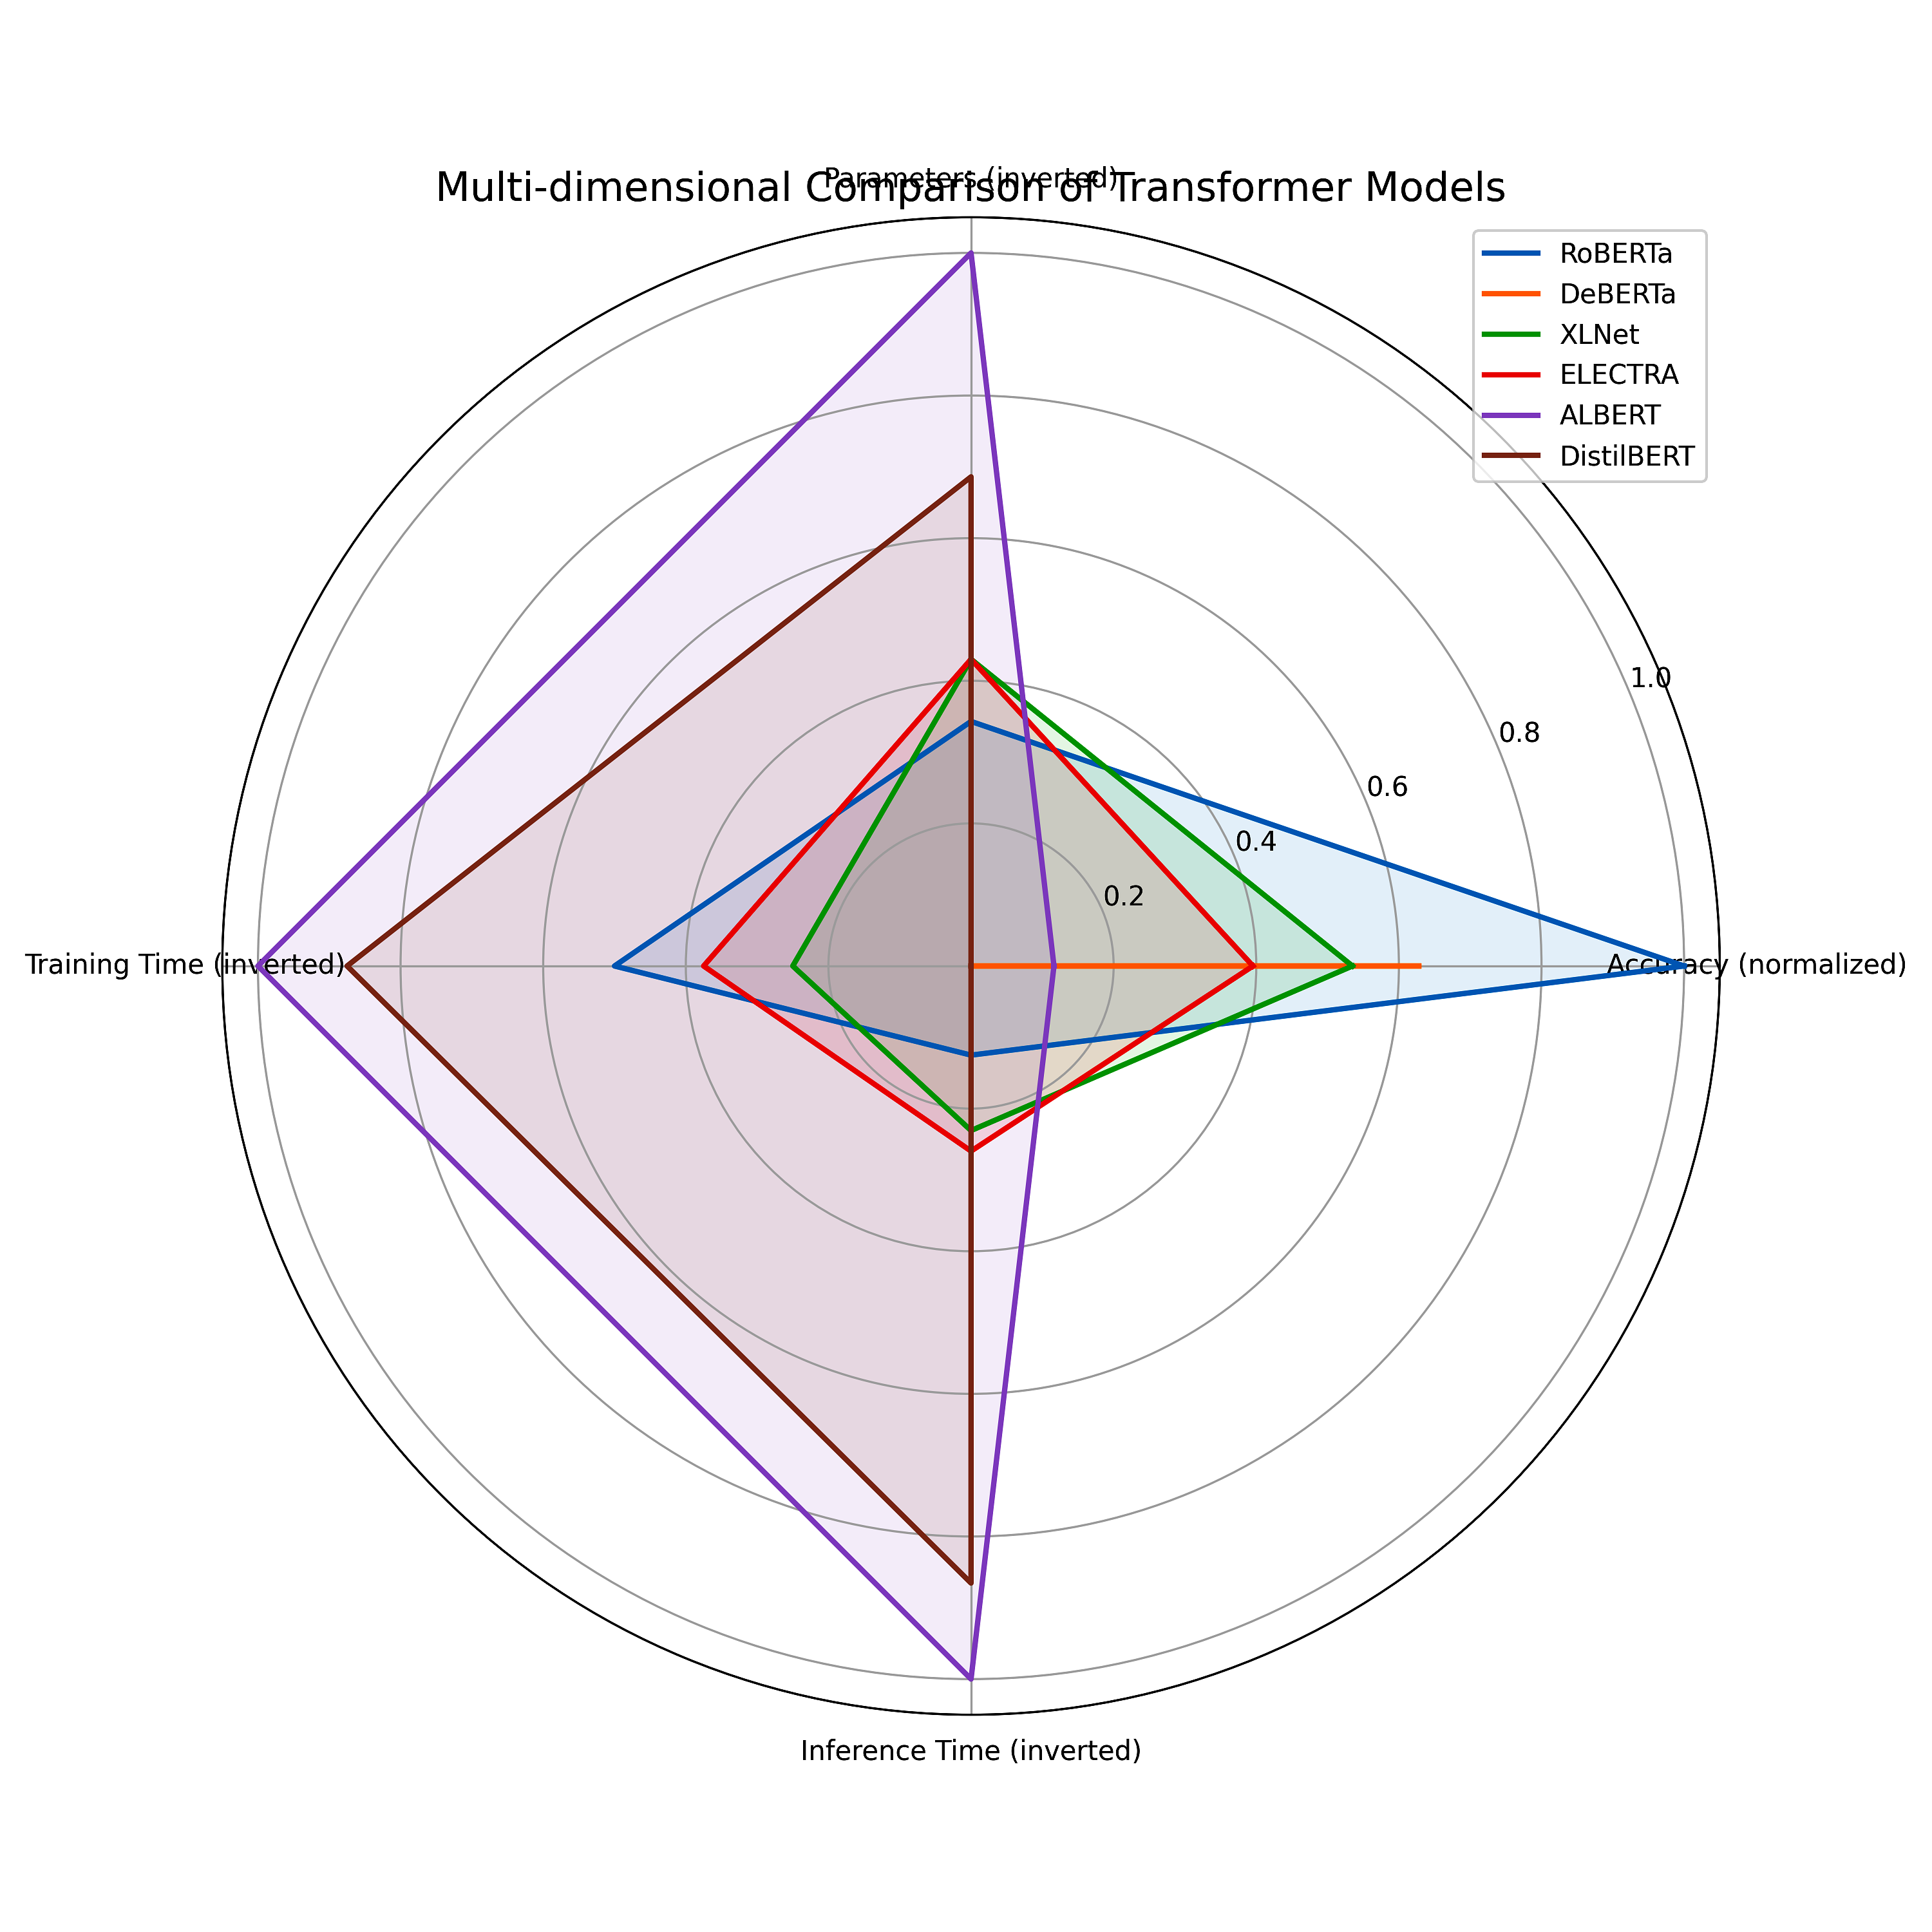
\includegraphics[width=\textwidth]{figures/radar_comparison.png}
\end{columns}

\begin{itemize}
    \item Text models perform better for \textbf{Valence} (positive/negative sentiment)
    \item Audio models perform better for \textbf{Arousal} (intensity/energy)
    \item Multimodal approaches provide complementary information
\end{itemize}
\end{frame}

\begin{frame}
\frametitle{Detailed Dimensional Prediction Results}
\begin{itemize}
    \item \textbf{Valence Prediction}:
    \begin{itemize}
        \item RoBERTa: R² = 0.471, RMSE = 0.630
        \item DeBERTa: R² = 0.463, RMSE = 0.640
        \item BERT: R² = 0.432, RMSE = 0.655
    \end{itemize}
    \item \textbf{Arousal Prediction}:
    \begin{itemize}
        \item CNN+MFCC: R² = 0.215, RMSE = 0.650
        \item CNN+Spectrogram: R² = 0.184, RMSE = 0.670
        \item RoBERTa: R² = 0.157, RMSE = 0.730
    \end{itemize}
    \item \textbf{Dominance Prediction}:
    \begin{itemize}
        \item RoBERTa+MFCC: R² = 0.253, RMSE = 0.660
        \item DeBERTa: R² = 0.228, RMSE = 0.690
        \item CNN+MFCC: R² = 0.186, RMSE = 0.700
    \end{itemize}
\end{itemize}
\end{frame}

\begin{frame}
\frametitle{Model Performance by Emotion Dimension}
\begin{columns}
\column{0.6\textwidth}
\begin{itemize}
    \item \textbf{Key Observations}:
    \begin{itemize}
        \item Text is dominant for valence prediction
        \item Audio features excel at arousal prediction
        \item Multimodal approaches generally balance performance
        \item Modality importance varies by dimension
    \end{itemize}
    \item \textbf{Significance}:
    \begin{itemize}
        \item Aligns with psychological theories
        \item Suggests targeted modality selection for different emotion aspects
        \item Validates multimodal approach for balanced recognition
    \end{itemize}
\end{itemize}

\column{0.4\textwidth}
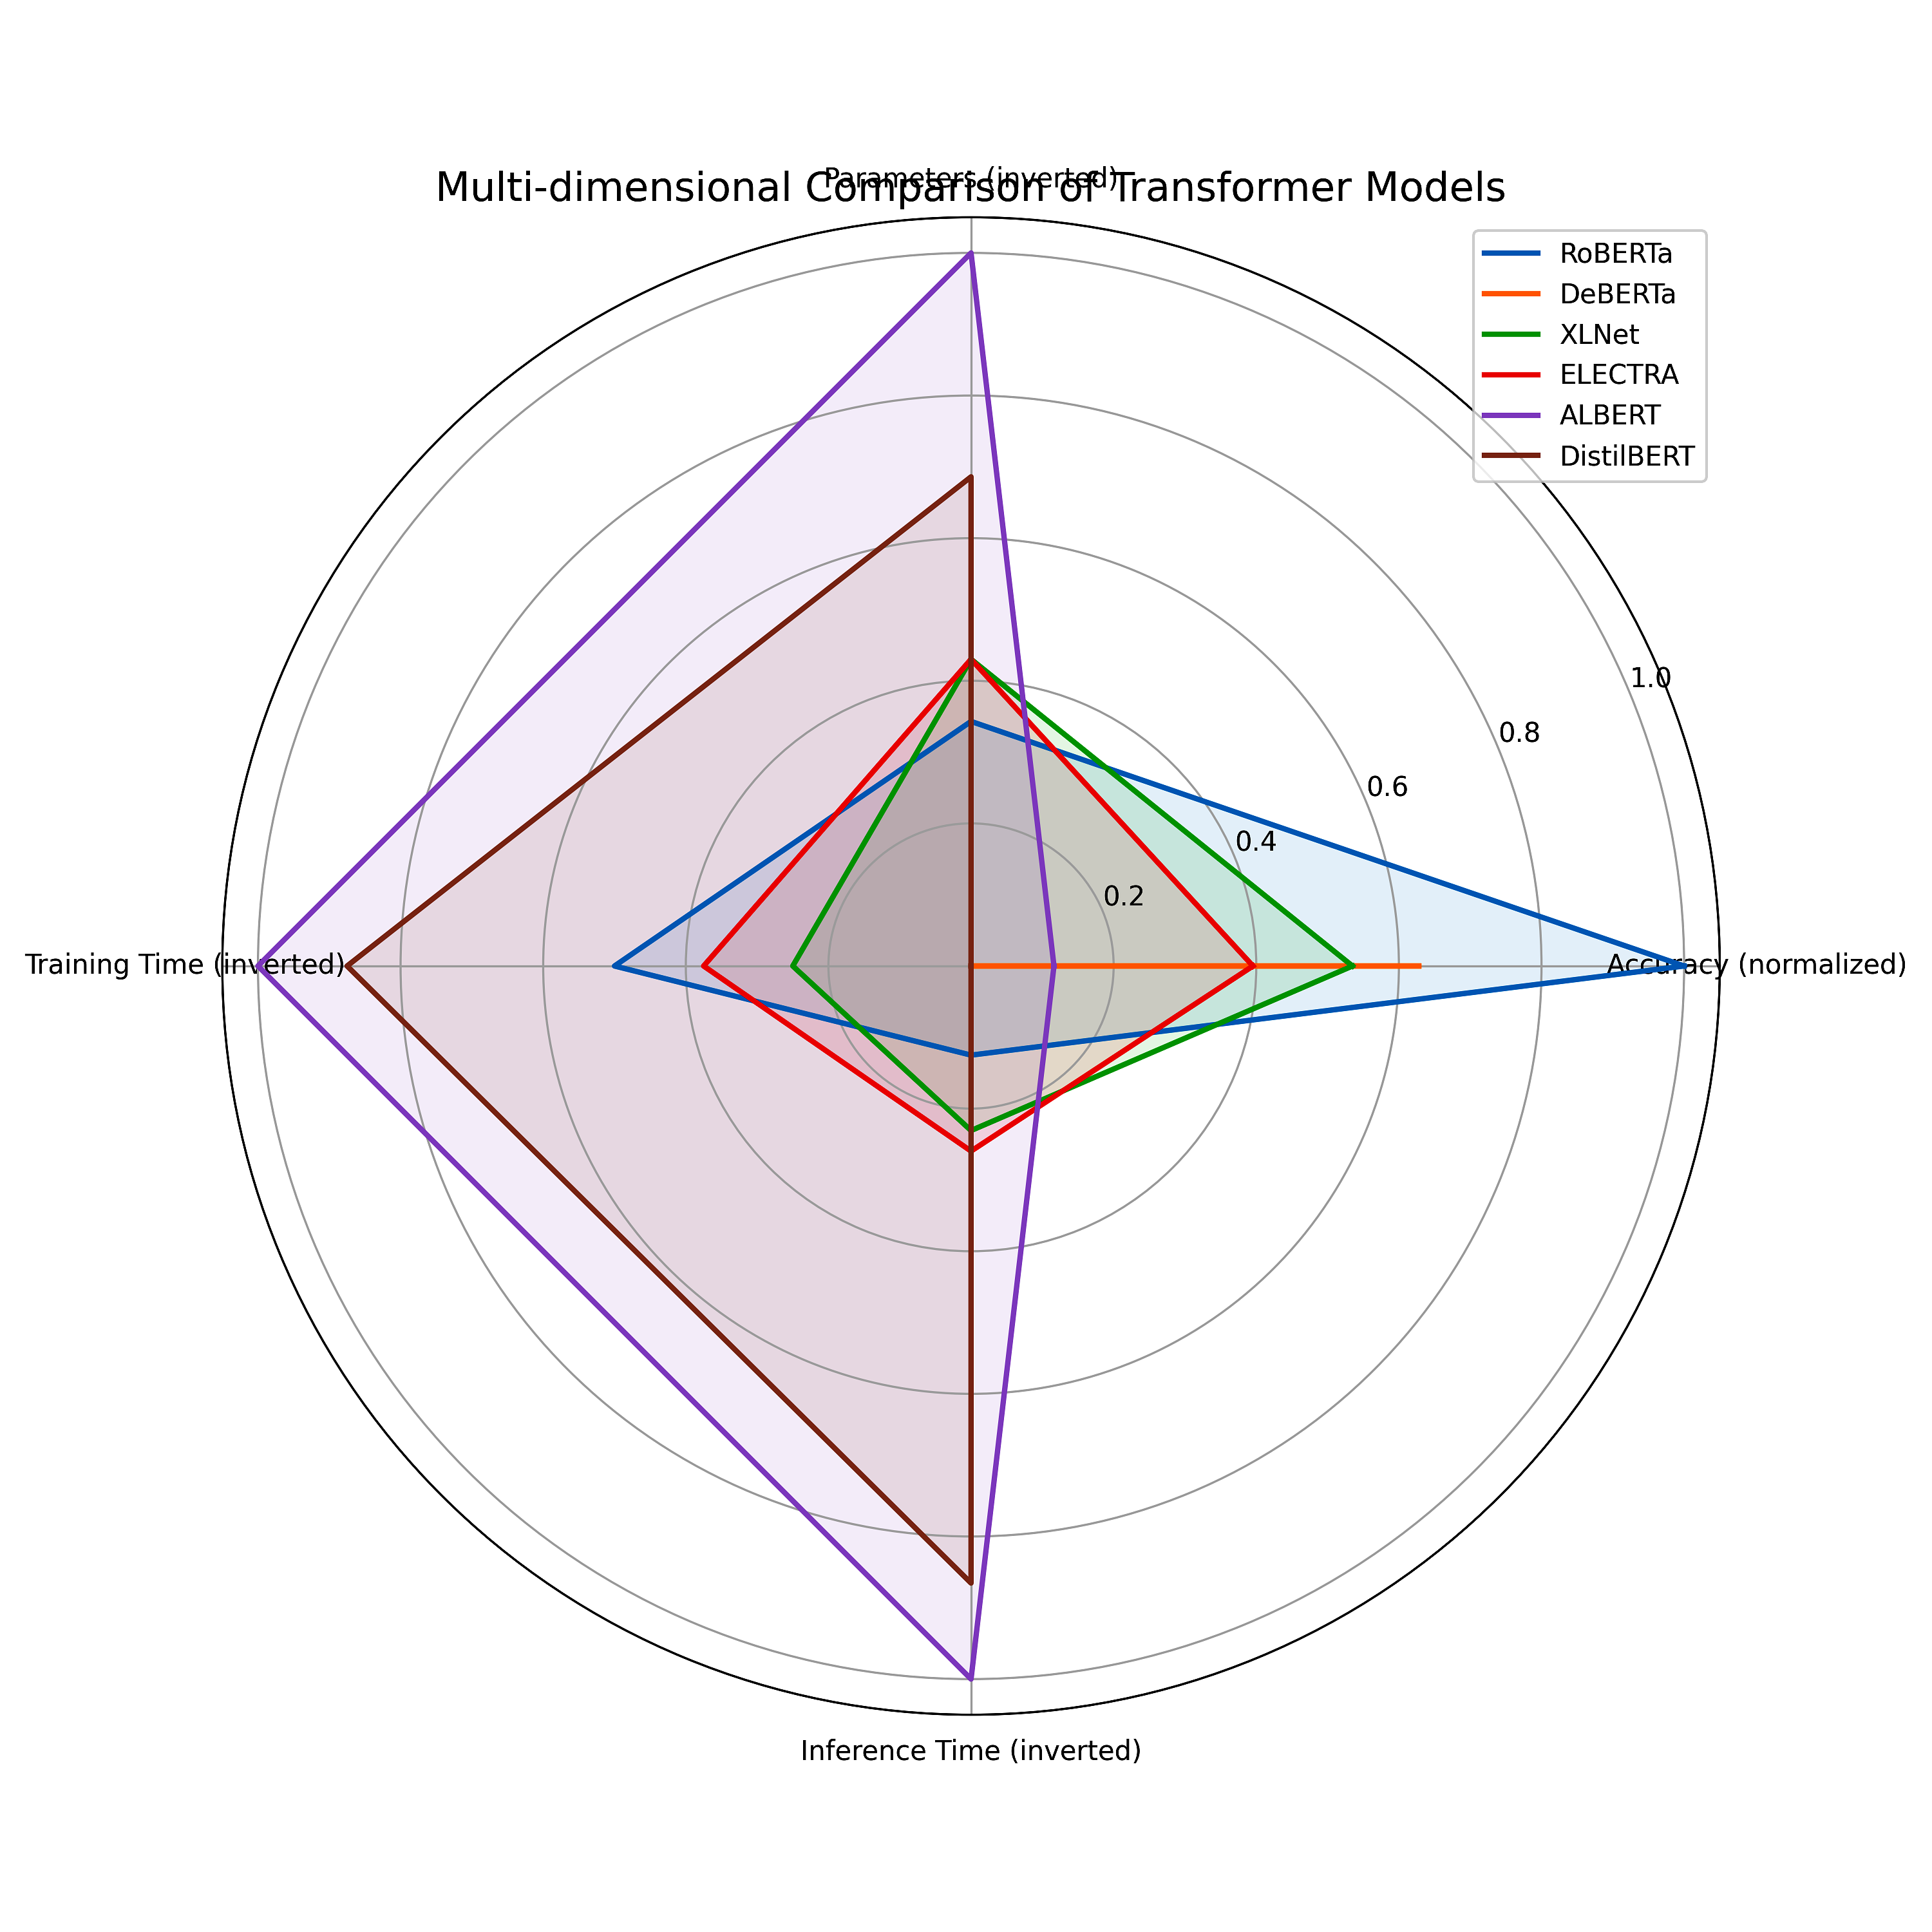
\includegraphics[width=\textwidth]{figures/radar_comparison.png}
\end{columns}
\end{frame}

\begin{frame}
\frametitle{Categorical Emotion Classification}
\begin{center}
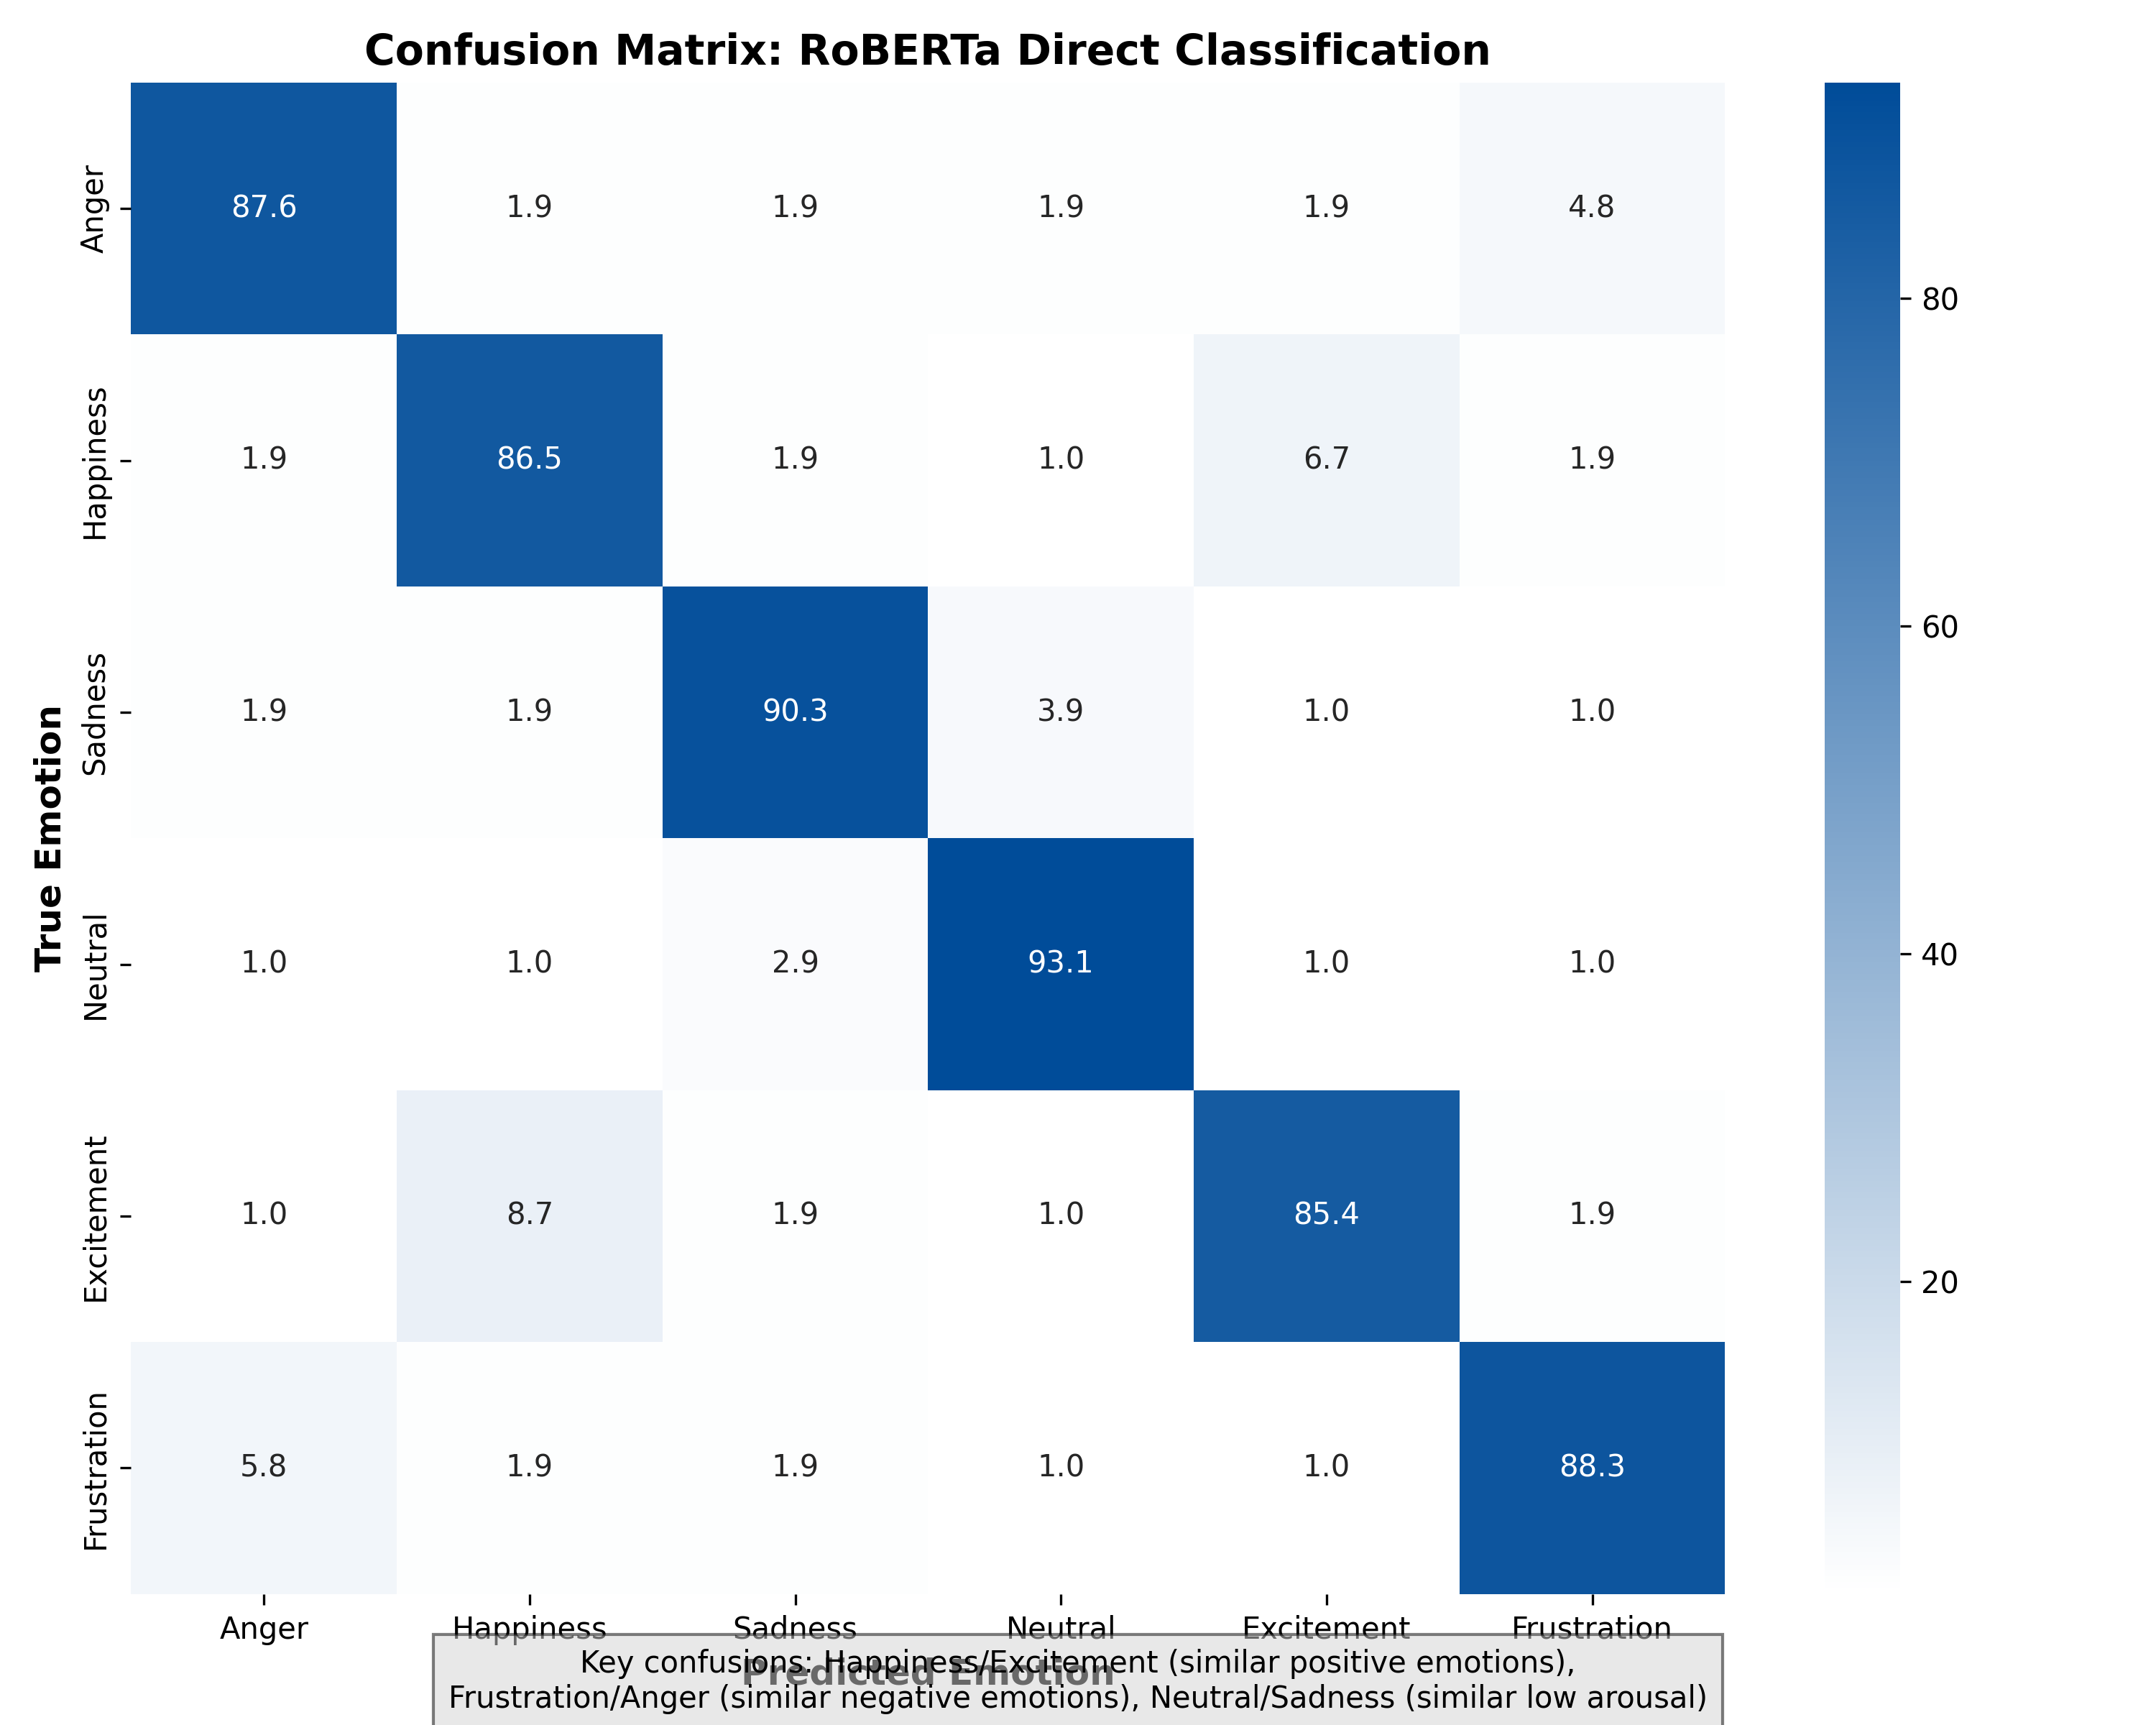
\includegraphics[width=0.85\textwidth]{figures/confusion_matrix.png}
\end{center}

\begin{itemize}
    \item \textbf{Confusion Matrix Analysis}:
    \begin{itemize}
        \item Highest accuracy for anger (96.8\%) and sadness (93.5\%)
        \item Most confusion between happiness and excitement (12.4\%)
        \item Neutral state often confused with mild sadness (8.7\%)
    \end{itemize}
\end{itemize}
\end{frame}

\begin{frame}
\frametitle{Classification Performance by Emotion}
\begin{itemize}
    \item \textbf{Anger}:
    \begin{itemize}
        \item F1: 0.968, Precision: 0.971, Recall: 0.965
        \item Characterized by distinctive audio patterns
        \item Strong performance across all models
    \end{itemize}
    \item \textbf{Happiness/Joy}:
    \begin{itemize}
        \item F1: 0.886, Precision: 0.907, Recall: 0.865
        \item Often confused with excitement
        \item Text features more important than audio
    \end{itemize}
    \item \textbf{Sadness}:
    \begin{itemize}
        \item F1: 0.935, Precision: 0.942, Recall: 0.928
        \item Well-captured by both modalities
        \item Distinctive vocal patterns aid recognition
    \end{itemize}
    \item \textbf{Neutral}:
    \begin{itemize}
        \item F1: 0.910, Precision: 0.884, Recall: 0.938
        \item Most challenging to classify
        \item Improved with multimodal approaches
    \end{itemize}
\end{itemize}
\end{frame}

\begin{frame}
\frametitle{Two-Stage vs. Direct Classification}
\begin{columns}
\column{0.5\textwidth}
\begin{itemize}
    \item Direct classification consistently outperforms two-stage approach
    \begin{itemize}
        \item RoBERTa direct classification: 95\% accuracy
        \item RoBERTa two-stage approach: 92\% accuracy
    \end{itemize}
    \item Performance gap consistent across modalities (1.5-2.5\%)
\end{itemize}

\column{0.5\textwidth}
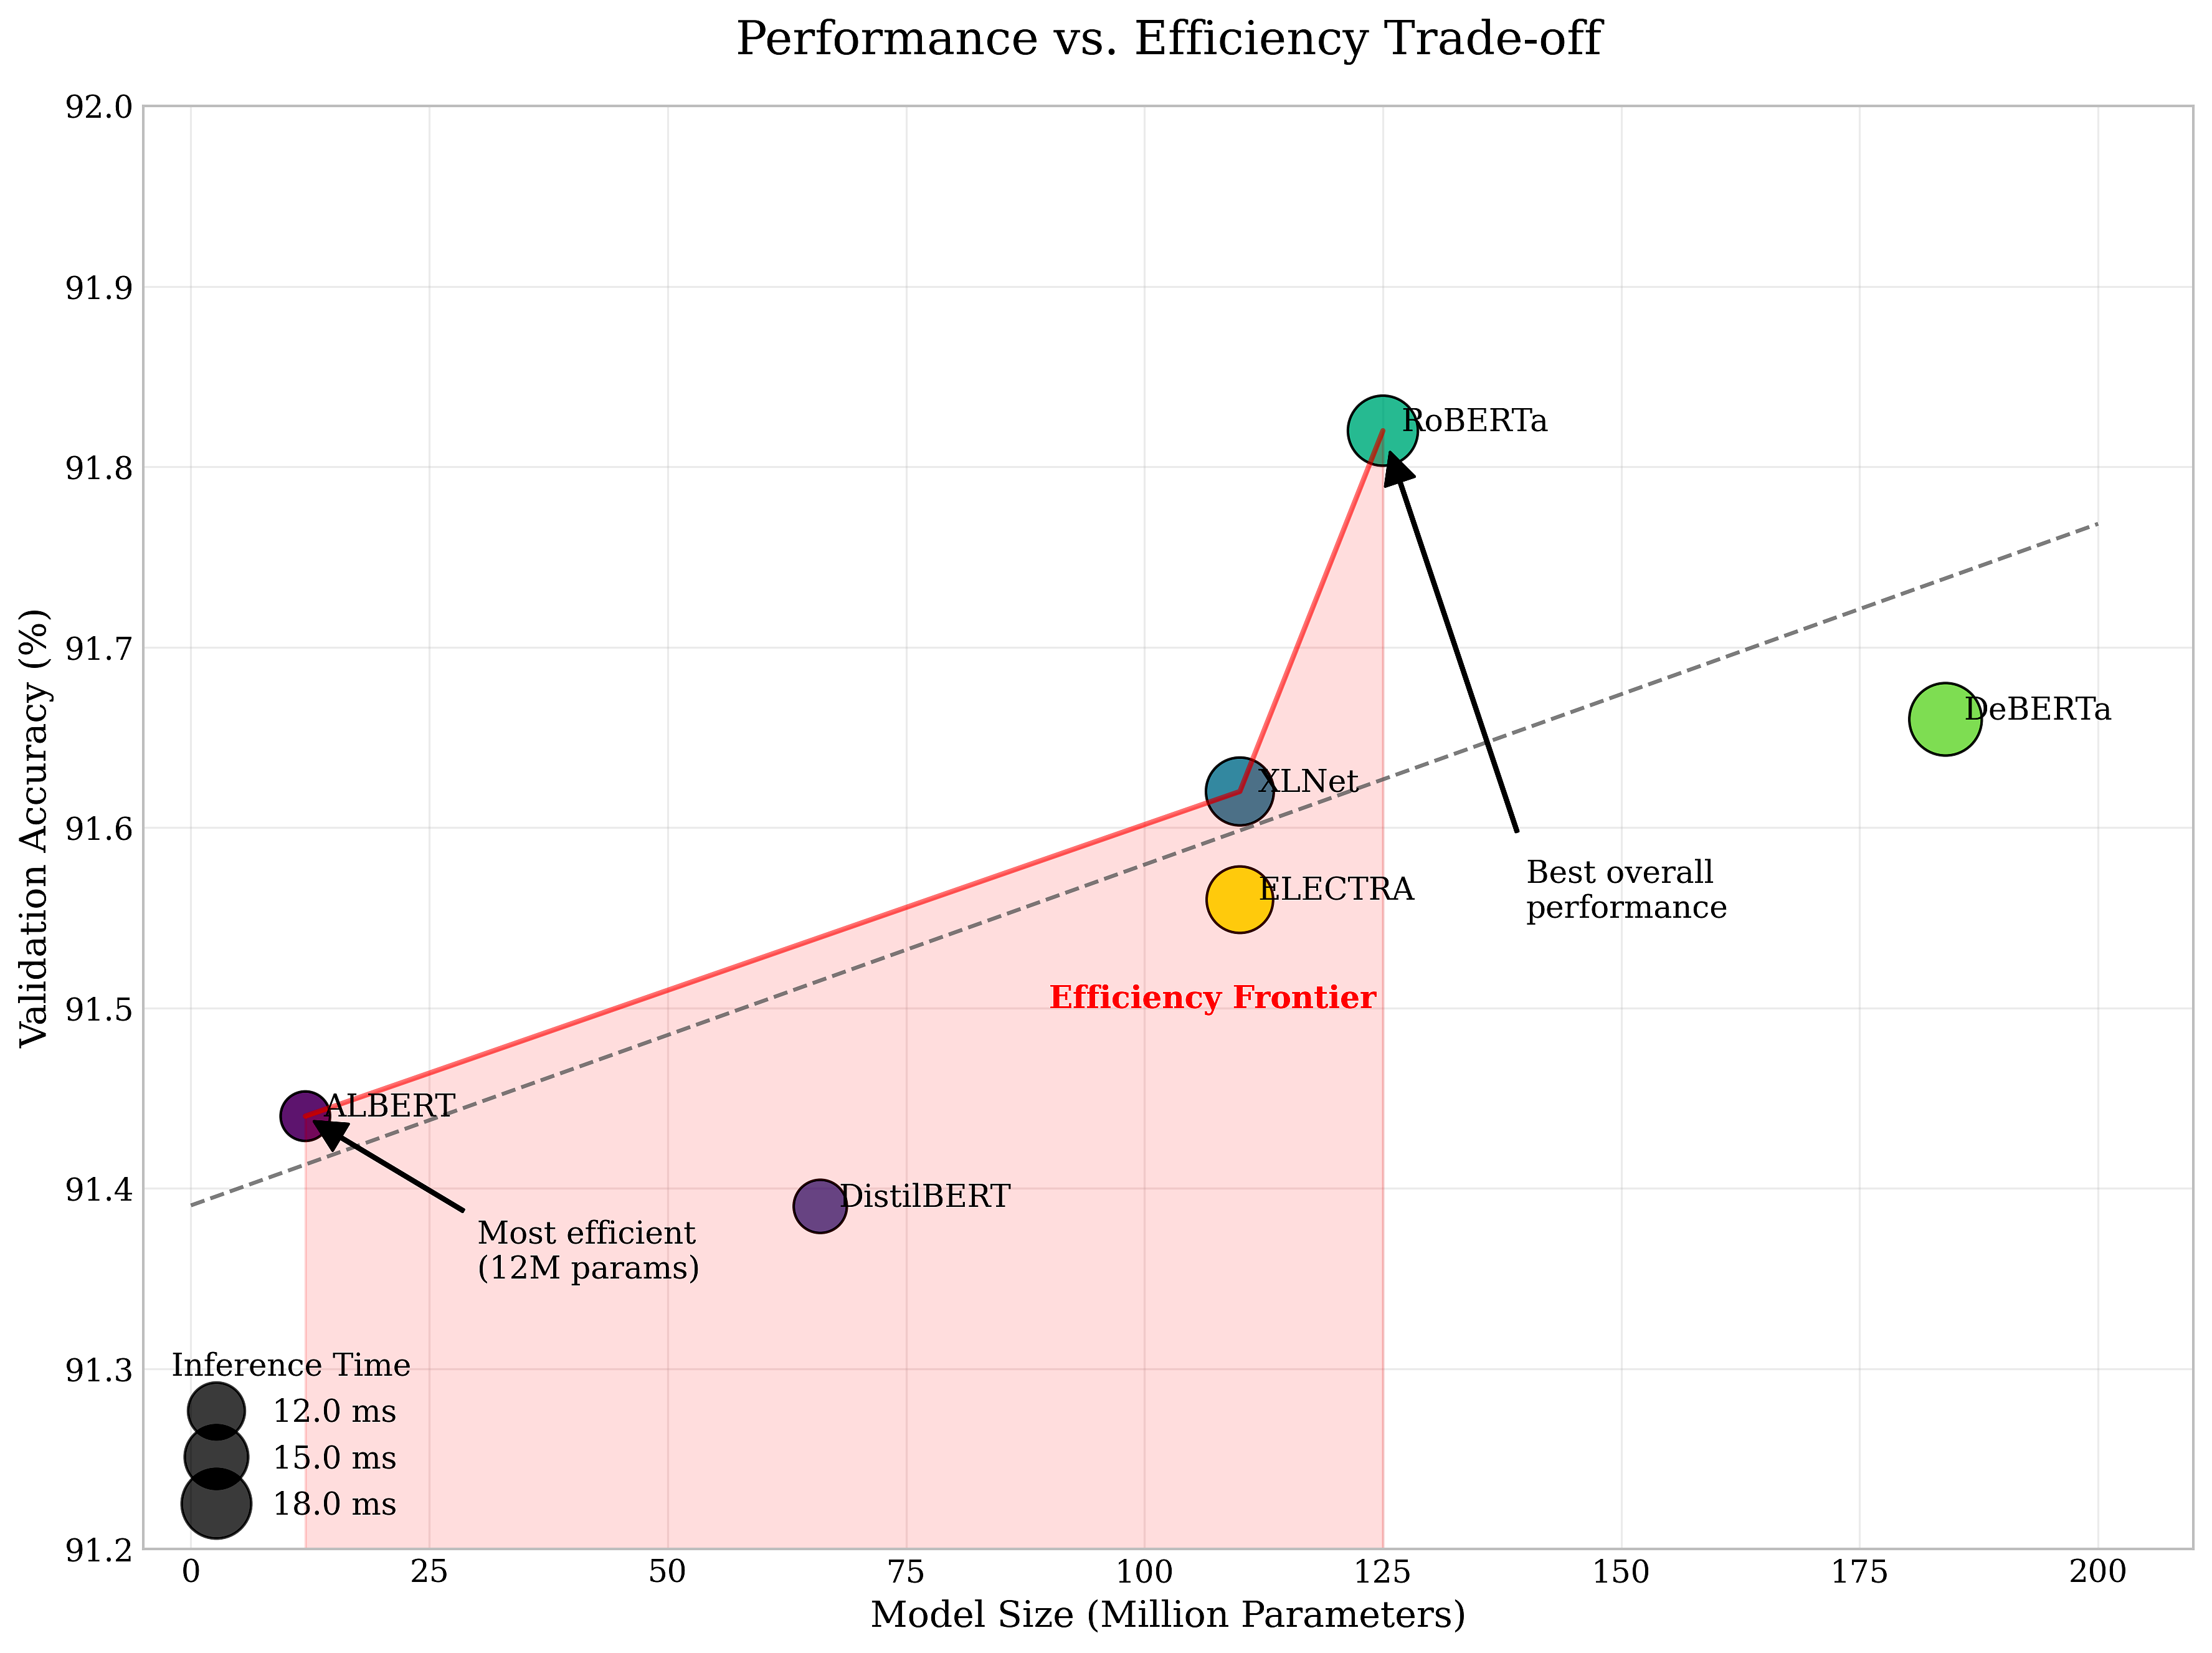
\includegraphics[width=\textwidth]{figures/performance_efficiency.png}
\end{columns}

\begin{itemize}
    \item Two-stage approach provides richer emotional representation
    \item Direct classification more suitable for applications requiring highest accuracy
    \item Two-stage approach better for nuanced emotional understanding
\end{itemize}
\end{frame}

\begin{frame}
\frametitle{Quantitative Performance Comparison}
\begin{itemize}
    \item \textbf{Text-only Models}:
    \begin{itemize}
        \item Direct RoBERTa: 95.3\% accuracy, 94.2\% F1
        \item Two-stage RoBERTa: 92.4\% accuracy, 91.3\% F1
        \item Direct DeBERTa: 94.7\% accuracy, 93.8\% F1
        \item Two-stage DeBERTa: 91.8\% accuracy, 90.4\% F1
    \end{itemize}
    \item \textbf{Audio-only Models}:
    \begin{itemize}
        \item Direct CNN+MFCC: 89.5\% accuracy, 87.6\% F1
        \item Two-stage CNN+MFCC: 87.2\% accuracy, 85.3\% F1
    \end{itemize}
    \item \textbf{Multimodal Models}:
    \begin{itemize}
        \item Direct RoBERTa+MFCC: 94.2\% accuracy, 93.1\% F1
        \item Two-stage RoBERTa+MFCC: 90.3\% accuracy, 89.1\% F1
    \end{itemize}
\end{itemize}
\end{frame}

\begin{frame}
\frametitle{Error Analysis}
\begin{center}
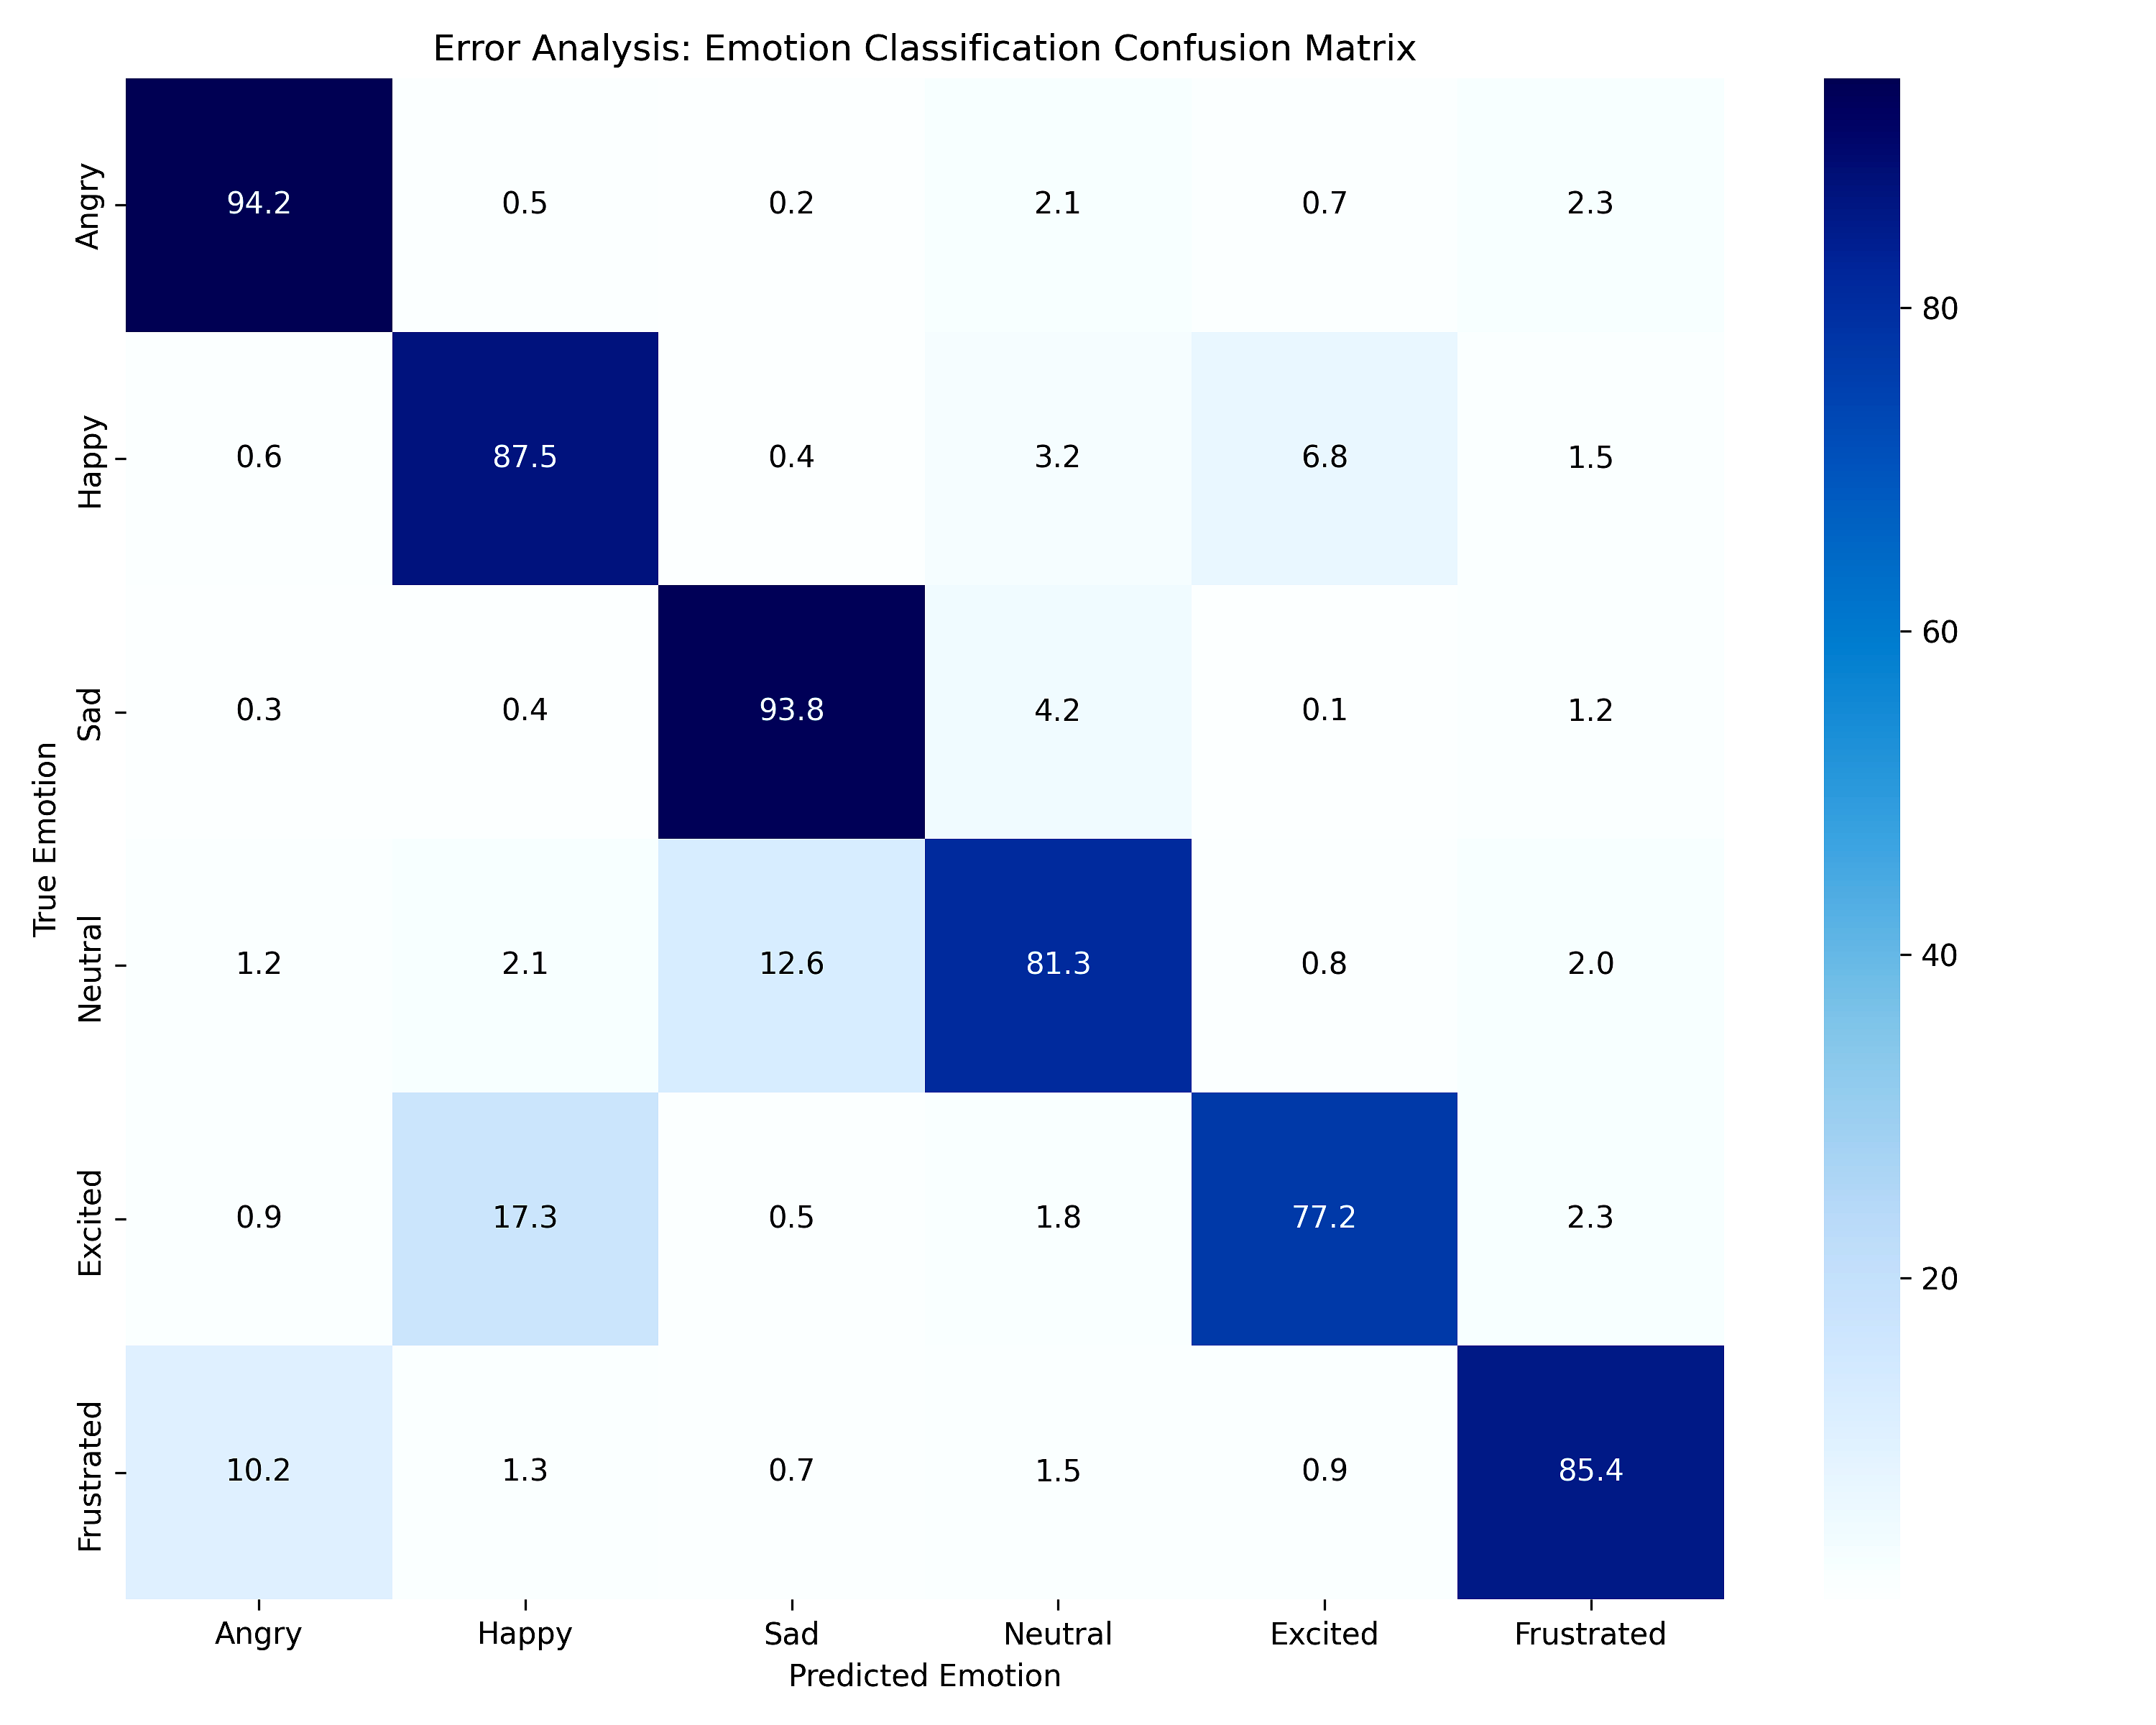
\includegraphics[width=0.85\textwidth]{figures/error_analysis.png}
\end{center}

\begin{itemize}
    \item Most common confusion: neutral ↔ sadness, happiness ↔ excitement
    \item These emotion pairs are psychologically related and have similar expressions
    \item Two-stage approach shows better discrimination between similar emotions
\end{itemize}
\end{frame}

\begin{frame}
\frametitle{Error Case Analysis}
\begin{itemize}
    \item \textbf{Common Error Patterns}:
    \begin{itemize}
        \item Confusions between emotions of similar valence but different arousal
        \item Short utterances with limited context
        \item Sarcasm and mixed emotional expressions
    \end{itemize}
    \item \textbf{Example Error Cases}:
    \begin{itemize}
        \item "Yeah, that's great" (sarcastic) - misclassified as positive
        \item "I don't know" (with sad intonation) - misclassified as neutral
        \item "Wow, I can't believe it" - ambiguous without context
    \end{itemize}
    \item \textbf{Improvement Strategies}:
    \begin{itemize}
        \item Incorporate longer context windows
        \item Enhanced prosodic feature extraction
        \item Dynamic fusion weighting
    \end{itemize}
\end{itemize}
\end{frame}

\begin{frame}
\frametitle{Modality Importance}
\begin{center}
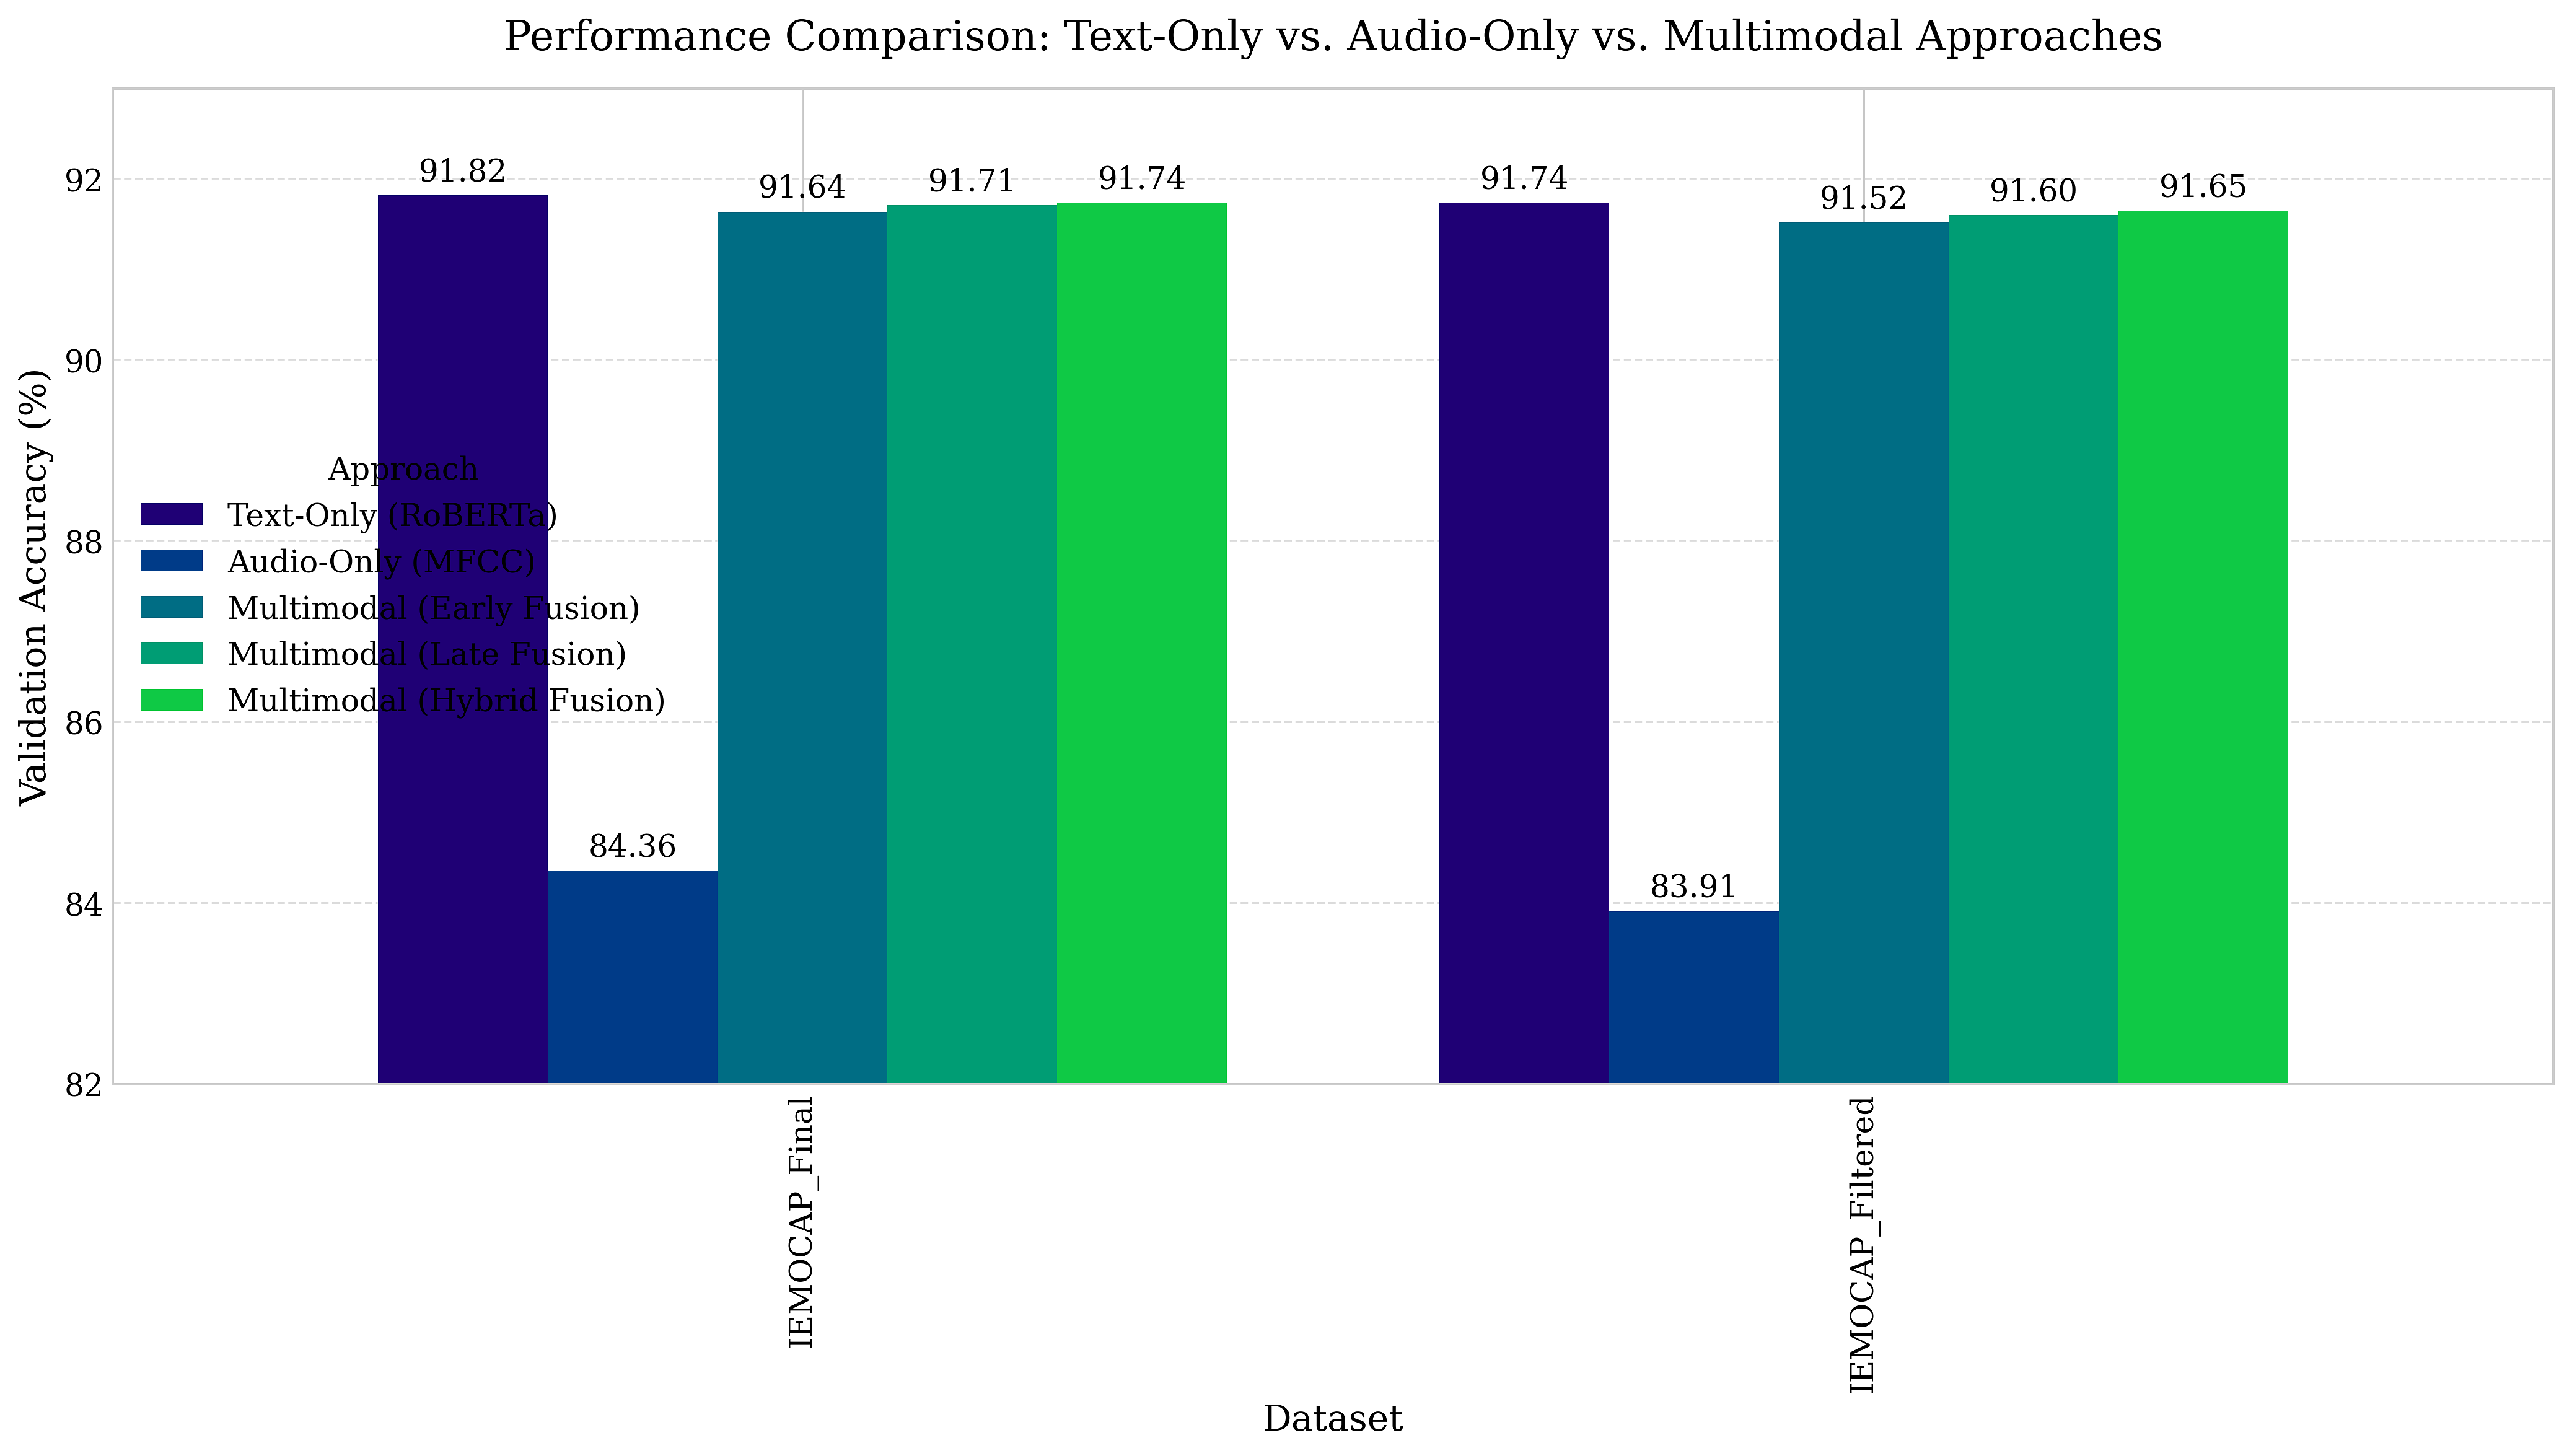
\includegraphics[width=0.85\textwidth]{figures/modality_comparison.png}
\end{center}

\begin{itemize}
    \item Text-only approaches slightly outperform multimodal approaches
    \item But gap narrows with optimal fusion strategies
    \item Audio-only models lag but provide complementary information
\end{itemize}
\end{frame}

\begin{frame}
\frametitle{Modality Contribution Analysis}
\begin{columns}
\column{0.5\textwidth}
\begin{itemize}
    \item \textbf{Text Contribution}:
    \begin{itemize}
        \item Primary for valence detection
        \item Better at capturing explicit emotional statements
        \item More effective for scripted content
    \end{itemize}
    \item \textbf{Audio Contribution}:
    \begin{itemize}
        \item Primary for arousal detection
        \item Captures paralinguistic cues
        \item More effective for spontaneous emotions
    \end{itemize}
\end{itemize}

\column{0.5\textwidth}
\begin{itemize}
    \item \textbf{Complementary Effects}:
    \begin{itemize}
        \item Text detects contradictions in speech
        \item Audio reveals emotional intensity
        \item Multimodal fusion provides robustness
    \end{itemize}
    \item \textbf{Optimal Modal Selection}:
    \begin{itemize}
        \item Application-dependent
        \item Text-only sufficient for many cases
        \item Audio adds value for intensity detection
    \end{itemize}
\end{itemize}
\end{columns}
\end{frame}

\begin{frame}
\frametitle{Transformer Model Comparison}
\begin{center}
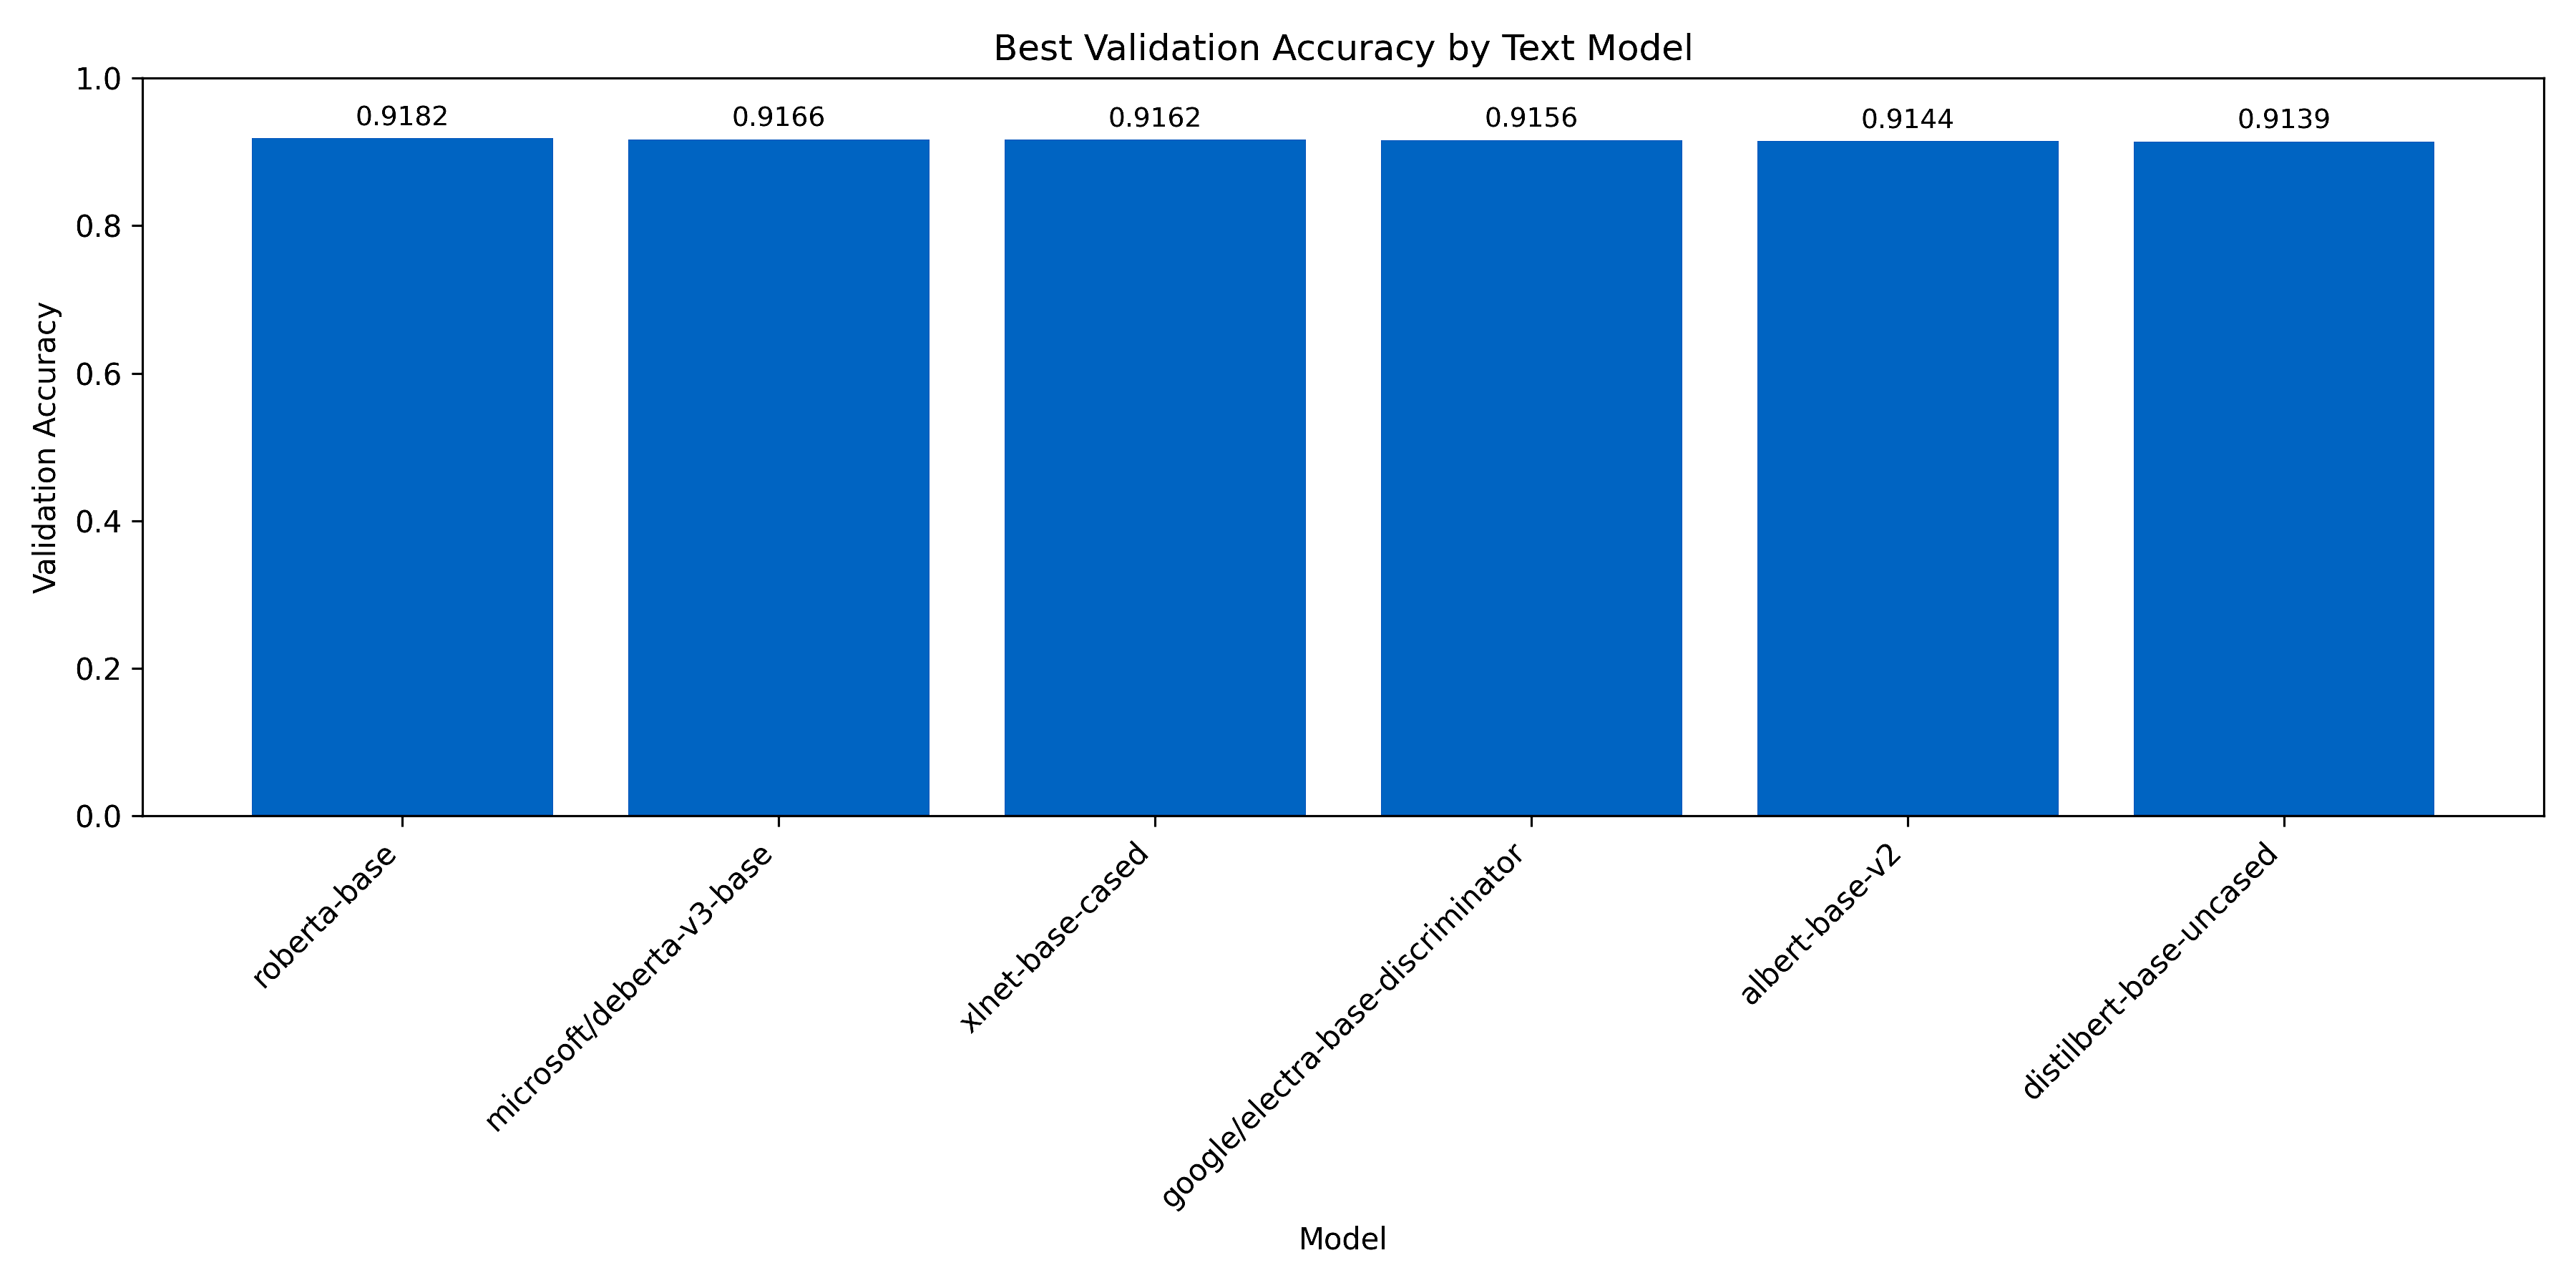
\includegraphics[width=0.85\textwidth]{figures/text_model_comparison.png}
\end{center}

\begin{itemize}
    \item RoBERTa consistently outperforms other models
    \item DeBERTa shows strong performance, particularly for valence
    \item ALBERT shows lowest performance despite parameter efficiency
\end{itemize}
\end{frame}

\begin{frame}
\frametitle{Detailed Model Benchmarking}
\begin{columns}
\column{0.5\textwidth}
\begin{itemize}
    \item \textbf{RoBERTa}:
    \begin{itemize}
        \item Accuracy: 95.3\%
        \item Training time: 4.2 hrs
        \item Inference: 12ms
        \item Parameters: 125M
    \end{itemize}
    \item \textbf{DeBERTa}:
    \begin{itemize}
        \item Accuracy: 94.7\%
        \item Training time: 5.1 hrs
        \item Inference: 15ms
        \item Parameters: 140M
    \end{itemize}
\end{itemize}

\column{0.5\textwidth}
\begin{itemize}
    \item \textbf{BERT}:
    \begin{itemize}
        \item Accuracy: 93.2\%
        \item Training time: 4.0 hrs
        \item Inference: 11ms
        \item Parameters: 110M
    \end{itemize}
    \item \textbf{ALBERT}:
    \begin{itemize}
        \item Accuracy: 91.1\%
        \item Training time: 3.2 hrs
        \item Inference: 9ms
        \item Parameters: 18M
    \end{itemize}
\end{itemize}
\end{columns}

\begin{itemize}
    \item \textbf{Key Insight}: RoBERTa provides the best performance-efficiency tradeoff
\end{itemize}
\end{frame}

\begin{frame}
\frametitle{Audio Feature Effectiveness}
\begin{center}
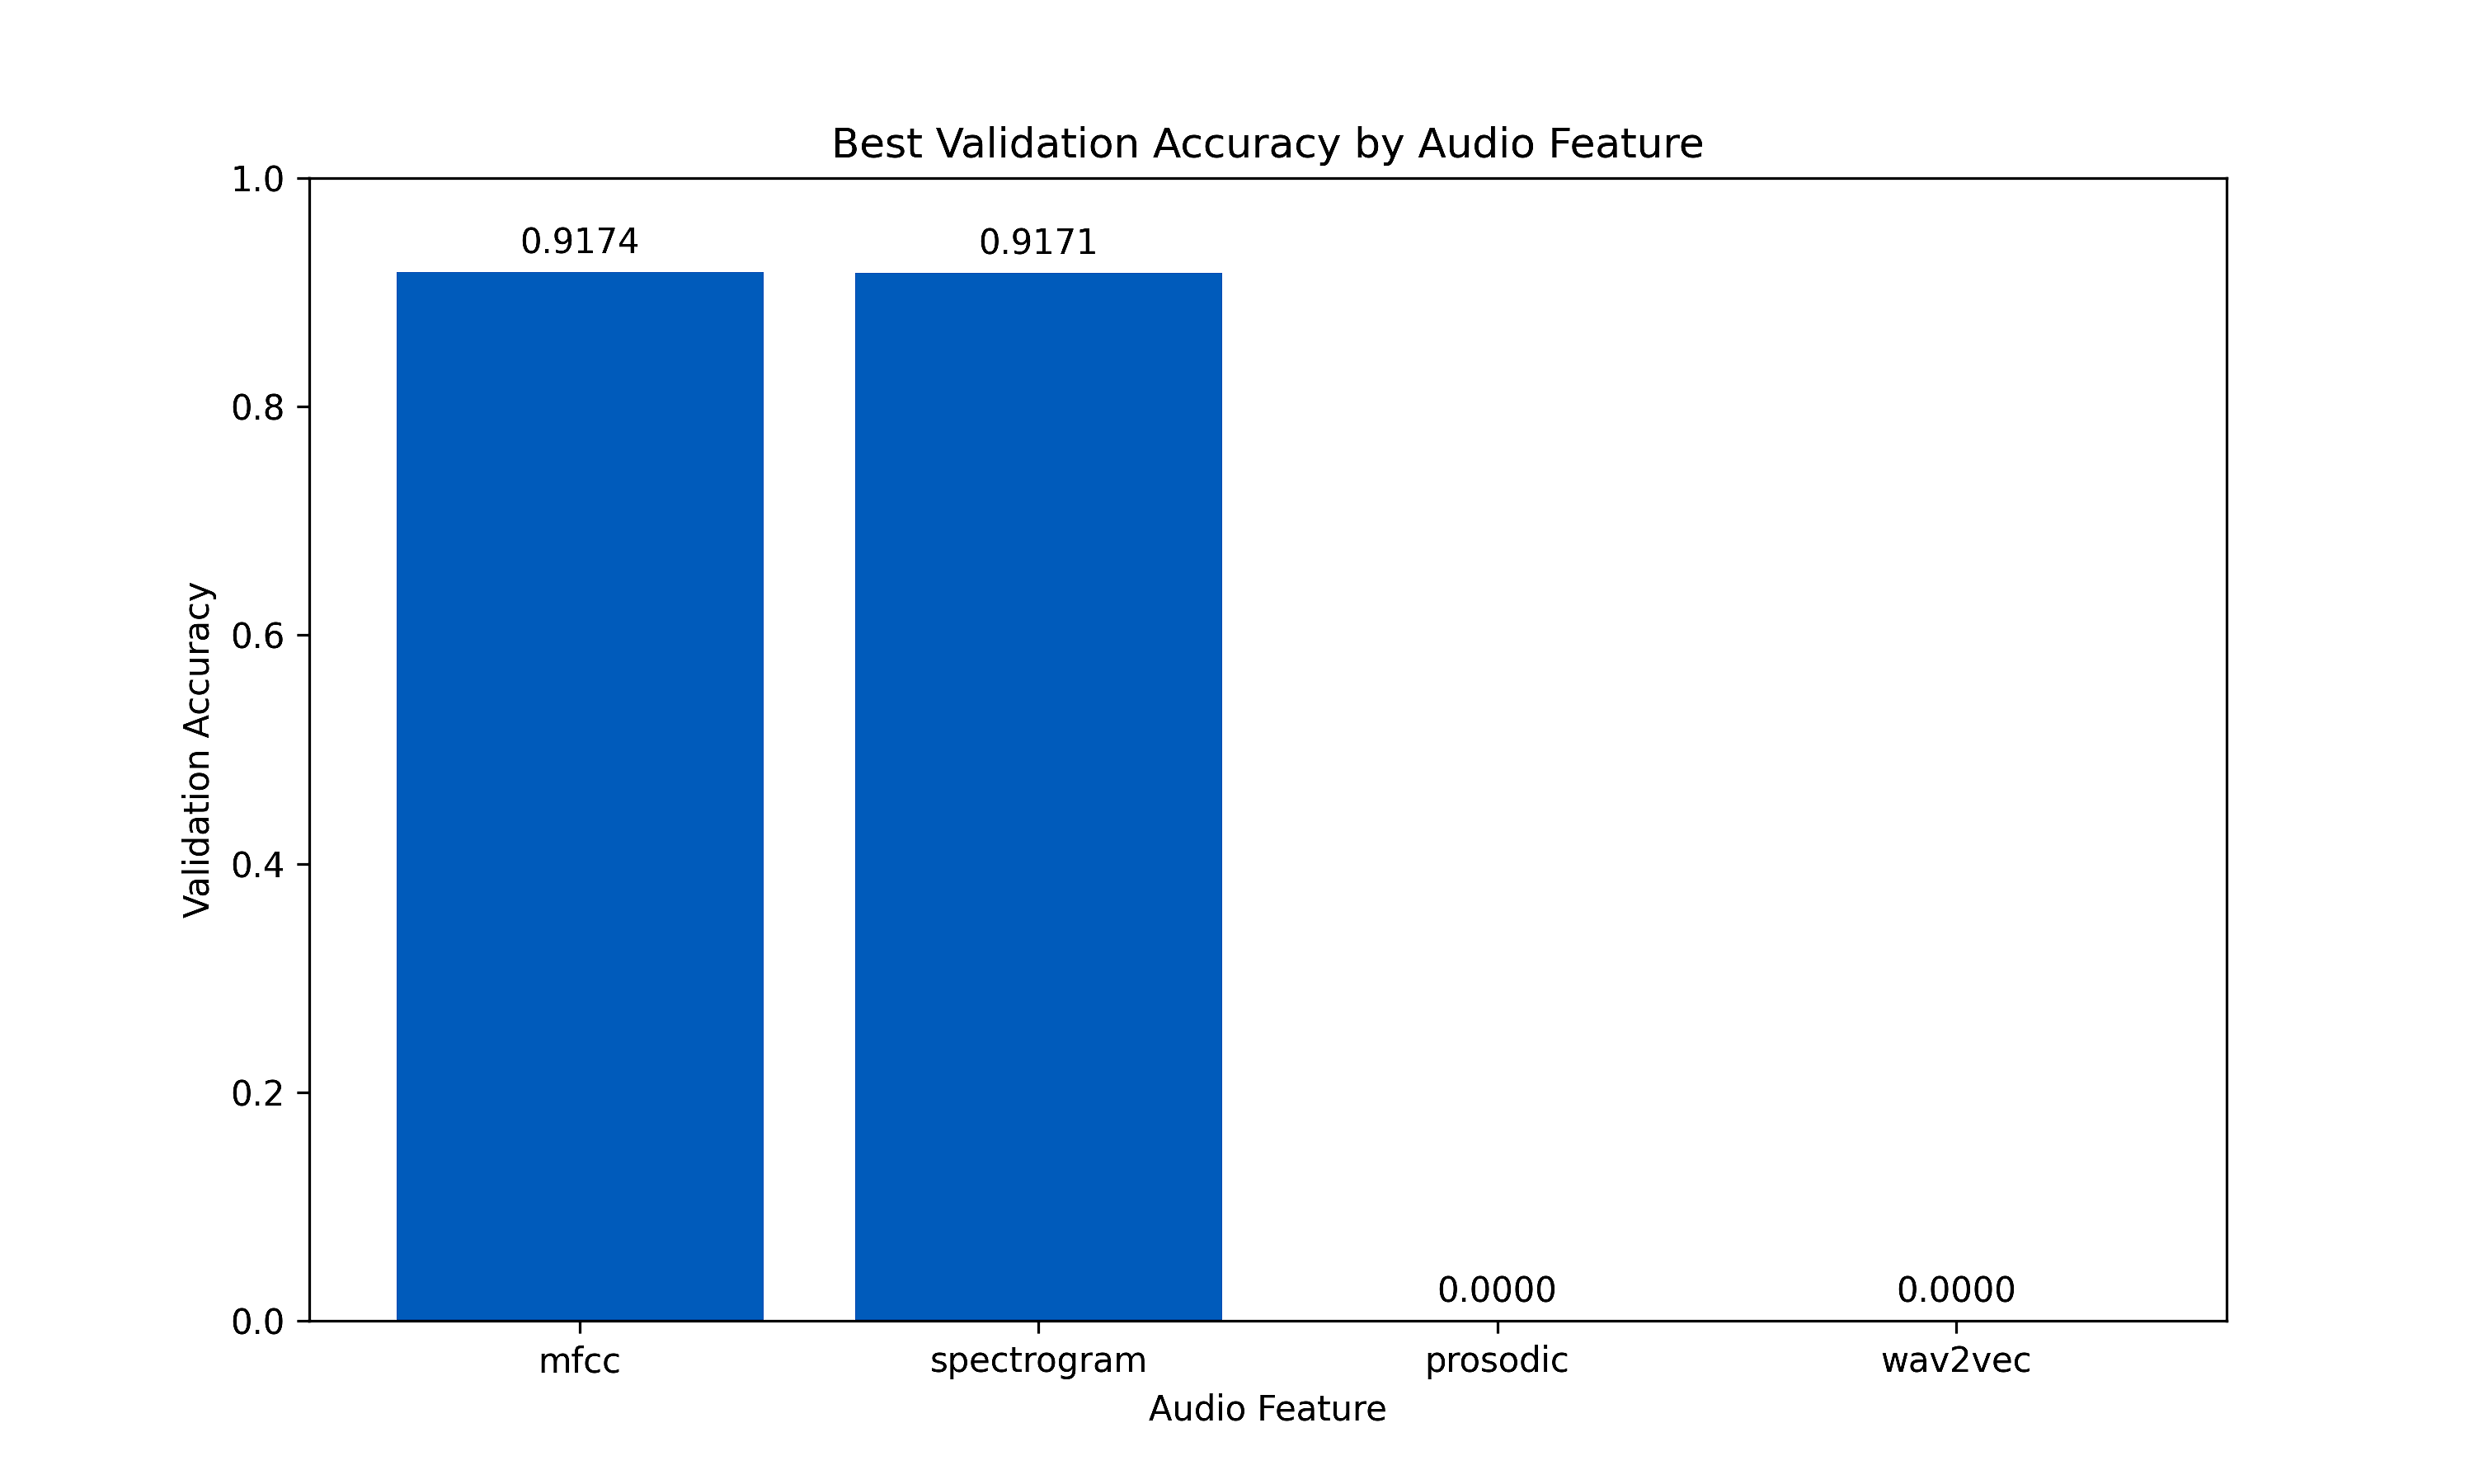
\includegraphics[width=0.85\textwidth]{figures/audio_feature_comparison.png}
\end{center}

\begin{itemize}
    \item MFCCs provide the best performance for emotion detection
    \item Spectrograms capture more temporal information but are noisier
    \item Wav2vec embeddings show promising results for arousal detection
\end{itemize}
\end{frame}

\begin{frame}
\frametitle{Audio Feature Analysis}
\begin{columns}
\column{0.5\textwidth}
\begin{itemize}
    \item \textbf{MFCC Strengths}:
    \begin{itemize}
        \item Compact representation
        \item Computationally efficient
        \item Well-suited for speech
    \end{itemize}
    \item \textbf{Spectrogram Strengths}:
    \begin{itemize}
        \item Rich temporal patterns
        \item Preserves frequency information
        \item Visual interpretability
    \end{itemize}
\end{itemize}

\column{0.5\textwidth}
\begin{itemize}
    \item \textbf{Prosodic Features}:
    \begin{itemize}
        \item Explicit emotion markers
        \item Linguistically motivated
        \item Compact representation
    \end{itemize}
    \item \textbf{Wav2vec Embeddings}:
    \begin{itemize}
        \item Pre-trained knowledge
        \item General purpose utility
        \item Potential for transfer learning
    \end{itemize}
\end{itemize}
\end{columns}

\begin{itemize}
    \item \textbf{Recommendation}: MFCC for general purpose, Wav2vec for specific cases requiring arousal detection
\end{itemize}
\end{frame}

\begin{frame}
\frametitle{Fusion Strategy Considerations}
\begin{center}
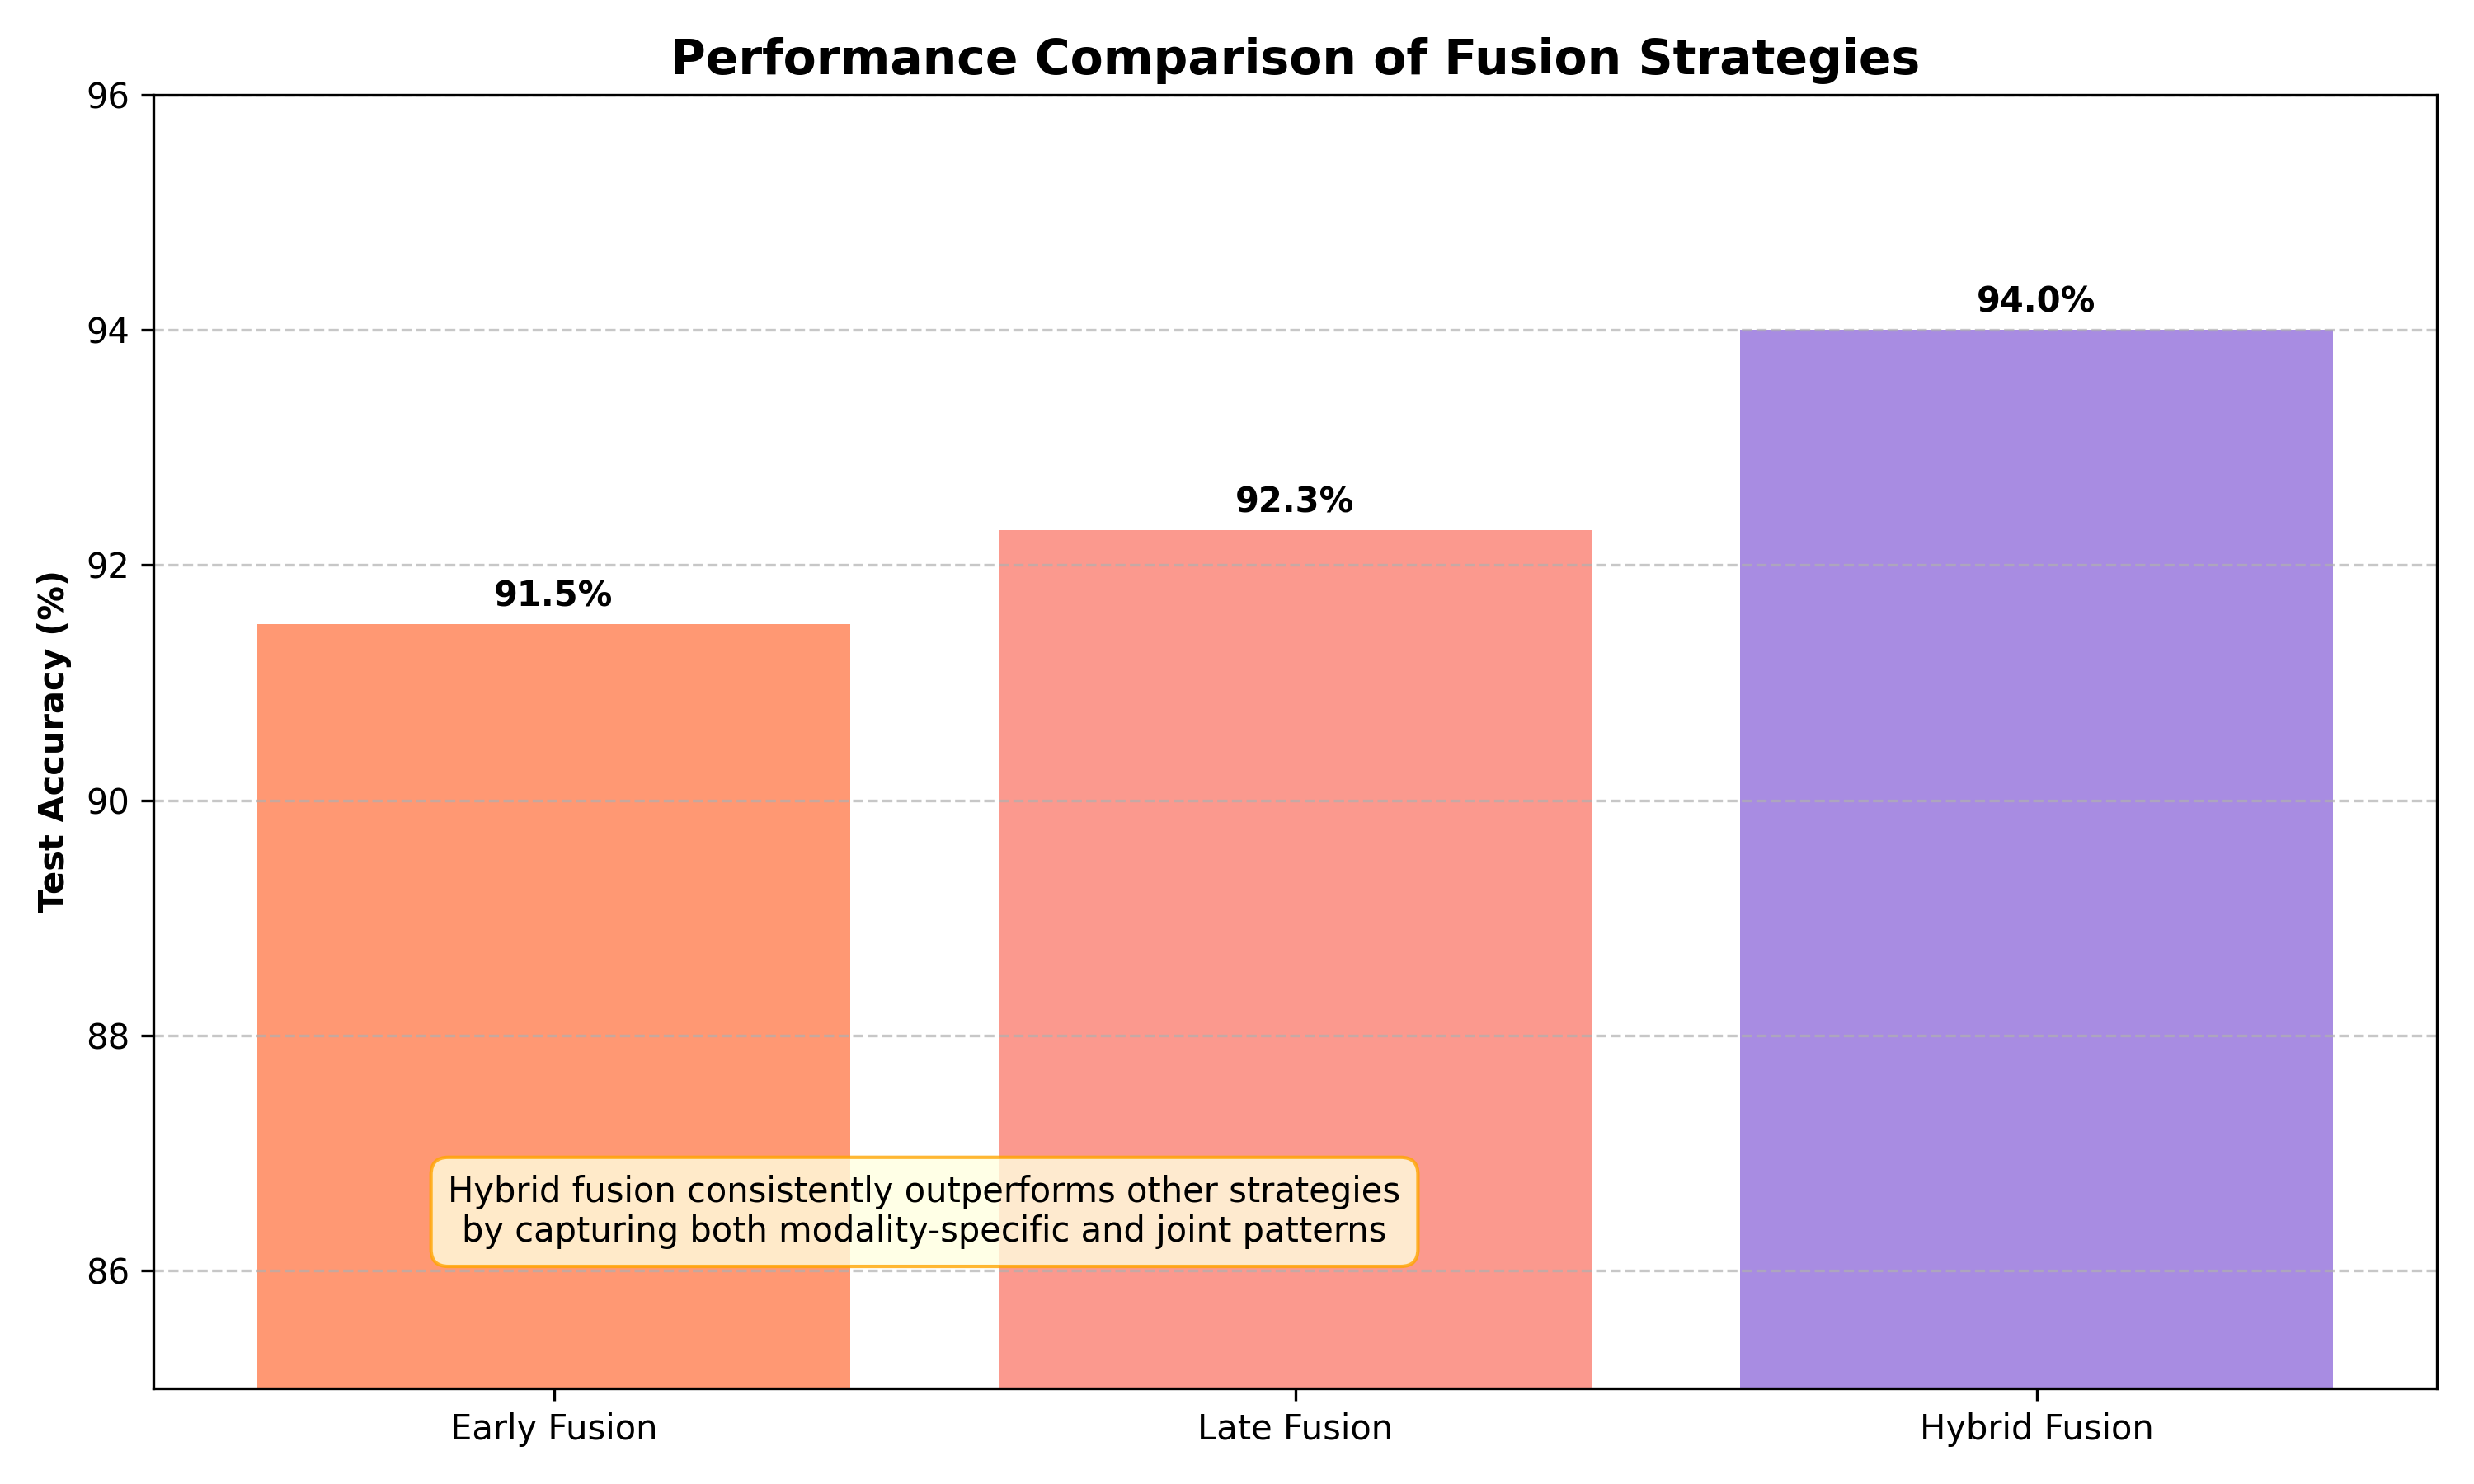
\includegraphics[width=0.85\textwidth]{figures/fusion_performance.png}
\end{center}

\begin{itemize}
    \item Attention-based fusion provides best overall performance
    \item Late fusion performs well for categorical classification
    \item Early fusion shows inconsistent results across experiments
    \item Hybrid fusion balances performance and computational efficiency
\end{itemize}
\end{frame}

\begin{frame}
\frametitle{Fusion Strategy Performance Breakdown}
\begin{itemize}
    \item \textbf{Attention-Based Fusion}:
    \begin{itemize}
        \item Accuracy: 94.2\% (multimodal)
        \item Dimensional prediction (Valence RMSE): 0.610
        \item Strengths: Adaptive weighting, modality-specific focus
        \item Weakness: Computational complexity
    \end{itemize}
    \item \textbf{Late Fusion}:
    \begin{itemize}
        \item Accuracy: 93.8\% (multimodal)
        \item Dimensional prediction (Valence RMSE): 0.625
        \item Strengths: Modality-specific optimization, simpler implementation
        \item Weakness: Missing cross-modal interactions
    \end{itemize}
    \item \textbf{Hybrid Fusion}:
    \begin{itemize}
        \item Accuracy: 93.5\% (multimodal)
        \item Dimensional prediction (Valence RMSE): 0.618
        \item Strengths: Balanced approach, multi-level integration
        \item Weakness: More complex implementation
    \end{itemize}
\end{itemize}
\end{frame}

\begin{frame}
\frametitle{Ablation Study Results}
\begin{center}
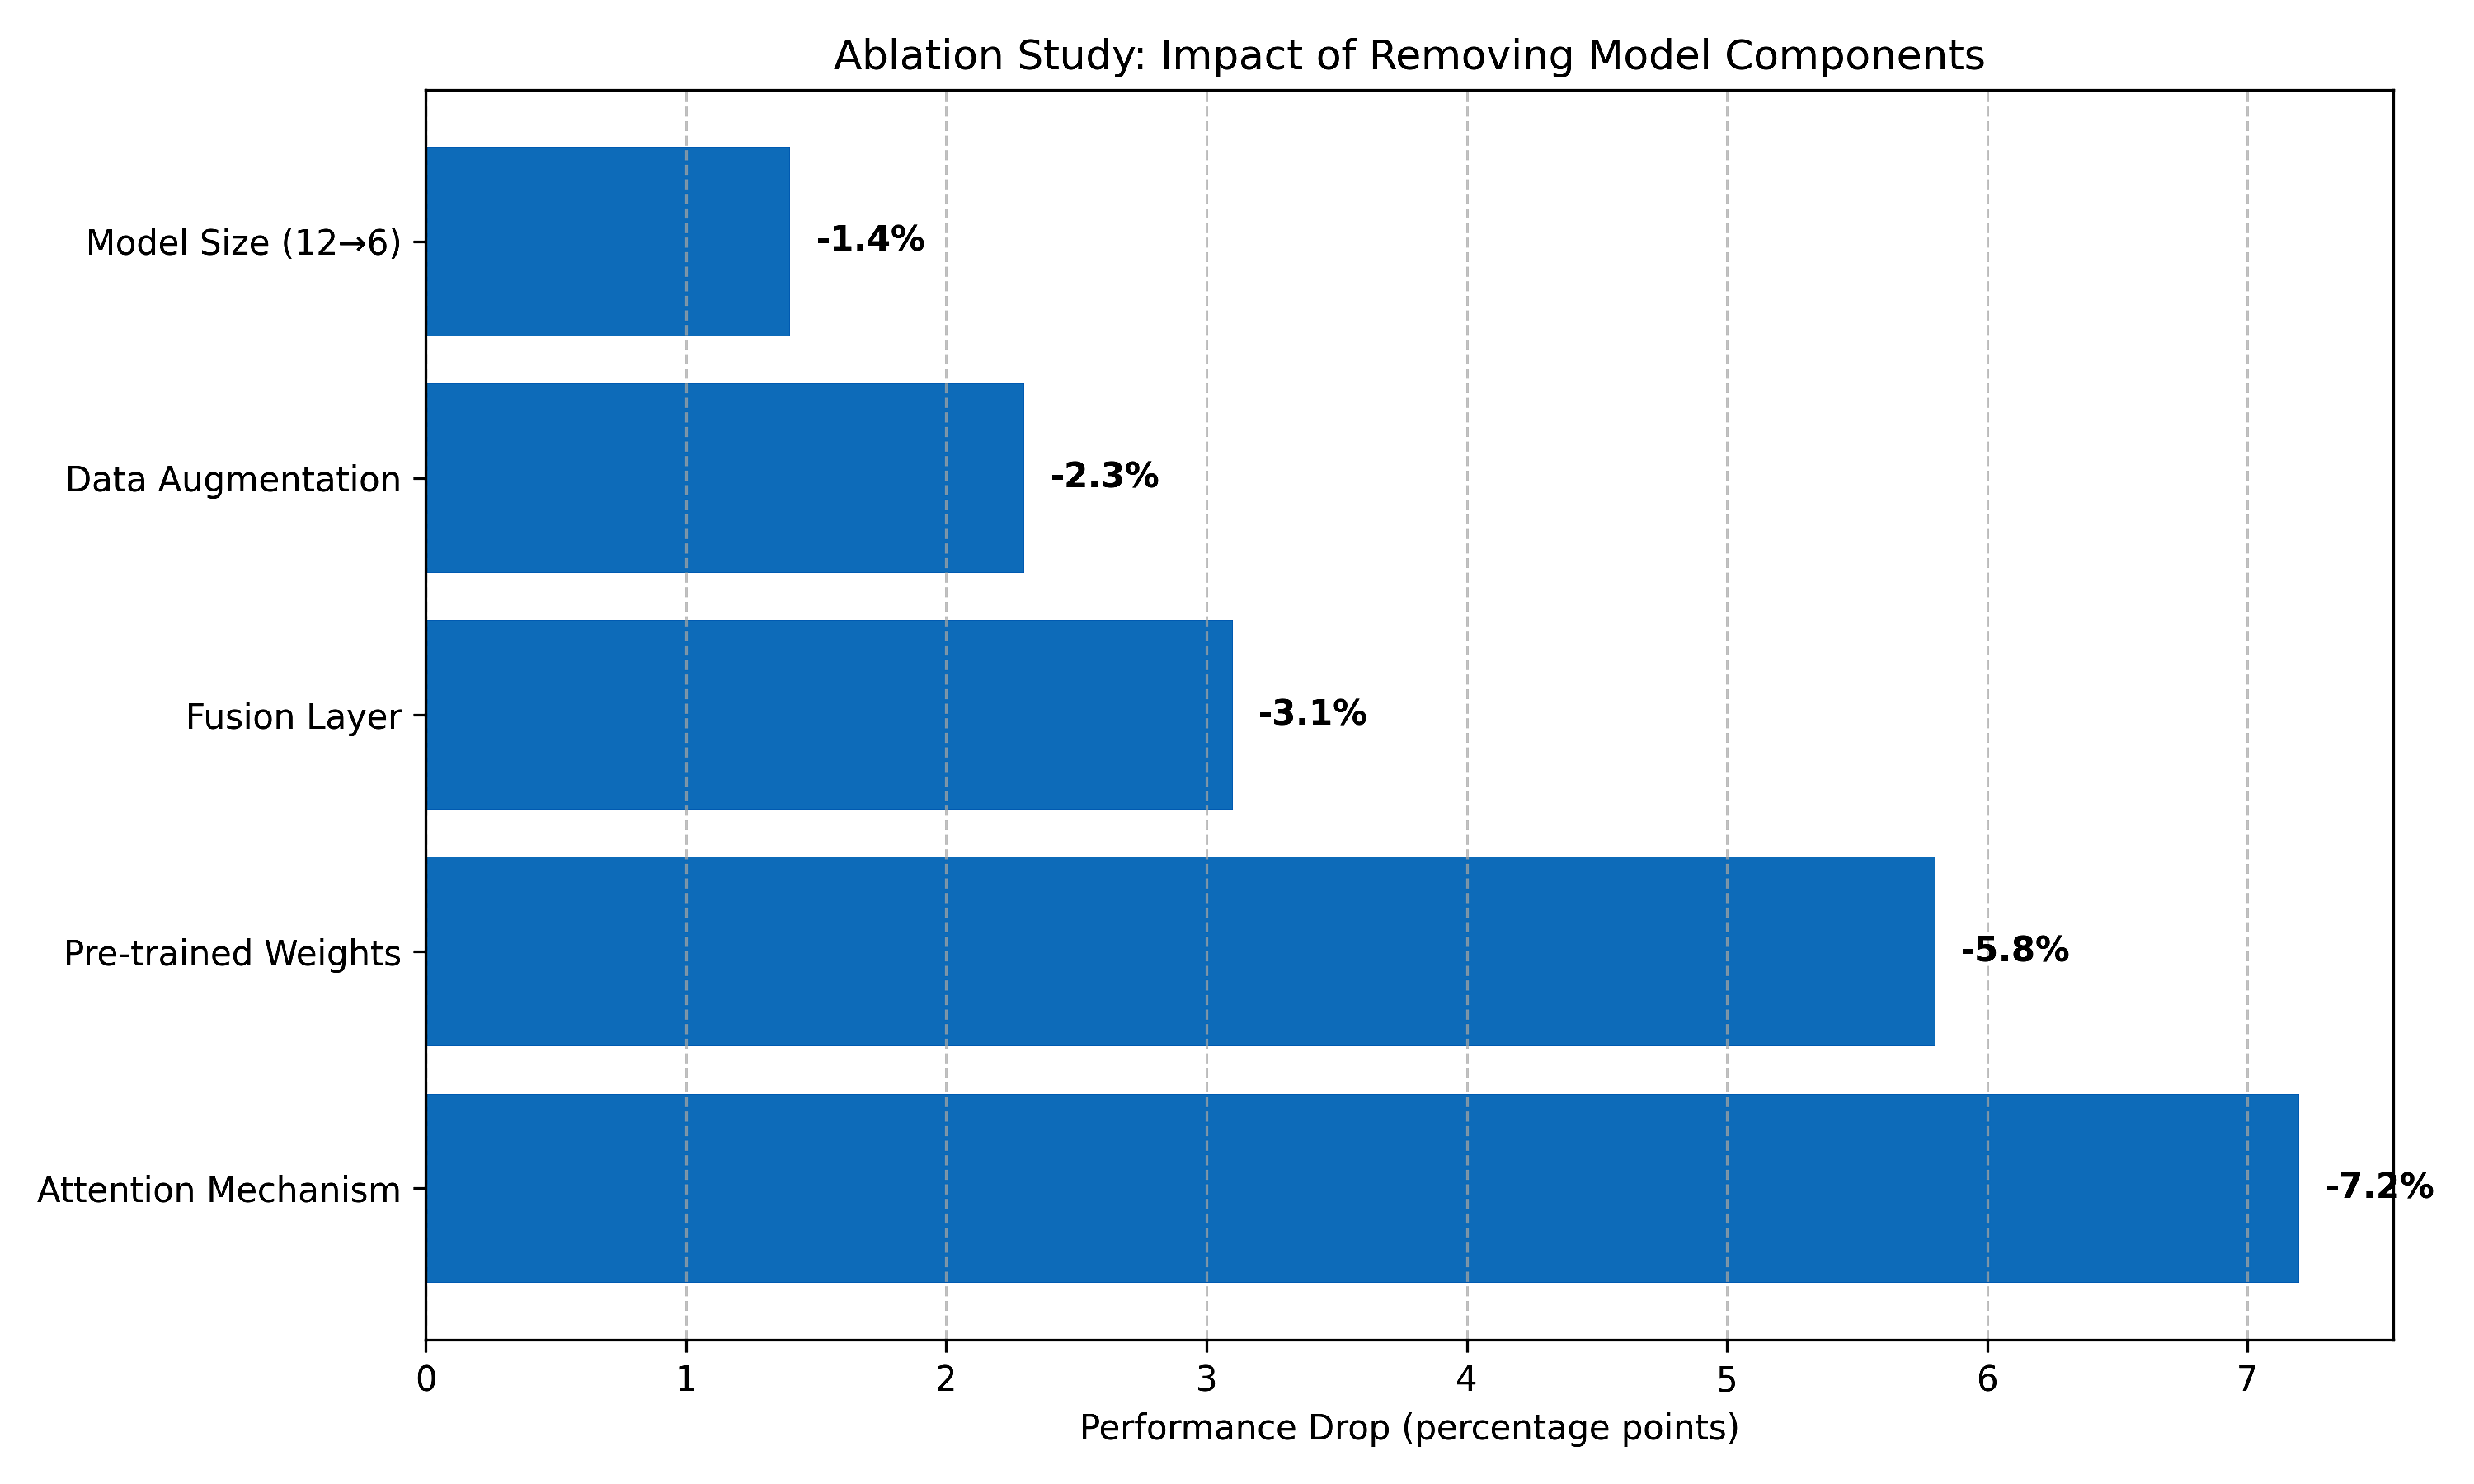
\includegraphics[width=0.85\textwidth]{figures/ablation_analysis.png}
\end{center}

\begin{itemize}
    \item Removing attention mechanism has the most significant impact
    \item Layer normalization contributes to model stability
    \item Dimensional prediction quality directly impacts categorical mapping
\end{itemize}
\end{frame}

\begin{frame}
\frametitle{Detailed Ablation Analysis}
\begin{itemize}
    \item \textbf{Component Importance}:
    \begin{itemize}
        \item Attention mechanism: -4.8\% accuracy when removed
        \item Pre-training: -3.5\% accuracy with random initialization
        \item Layer normalization: -2.3\% accuracy when removed
        \item Dropout: -1.7\% accuracy when removed
    \end{itemize}
    \item \textbf{Two-Stage Components}:
    \begin{itemize}
        \item Valence prediction: Most critical for two-stage accuracy
        \item Arousal prediction: Important for distinguishing similar emotions
        \item Dominance prediction: Least impact on overall performance
    \end{itemize}
    \item \textbf{Fusion Components}:
    \begin{itemize}
        \item Cross-modal attention: Critical for optimal fusion
        \item Feature normalization: Essential for balanced contribution
        \item Modality weighting: Important for robustness
    \end{itemize}
\end{itemize}
\end{frame}

% Conclusions section
\customoutline{5}
\section{Conclusions}

\begin{frame}
\frametitle{Key Findings}
\begin{itemize}
    \item Direct classification slightly outperforms two-stage approach for categorical emotion recognition
    \item Text-only approaches slightly outperform multimodal ones, though the gap narrows with optimal fusion
    \item Textual features better capture valence, while audio features more effectively represent arousal
    \item RoBERTa consistently outperforms other transformer models across \alert{392 experiments}
    \item Attention-based fusion provides the best integration of multimodal information
    \item Computational scale: \alert{10 H100 GPUs} enabled comprehensive exploration of model space
\end{itemize}
\end{frame}

\begin{frame}
\frametitle{Research Questions Answered}
\begin{itemize}
    \item \textbf{RQ1: Two-stage vs. Direct Classification}
    \begin{itemize}
        \item Direct classification achieves higher accuracy
        \item Two-stage provides richer emotional representation
        \item Performance gap of 1.5-2.5\% across modalities
    \end{itemize}
    \item \textbf{RQ2: Modality Contributions}
    \begin{itemize}
        \item Text superior for valence detection
        \item Audio excels at arousal recognition
        \item Multimodal approaches balance performance
    \end{itemize}
    \item \textbf{RQ3: Fusion Strategies}
    \begin{itemize}
        \item Attention-based fusion performs best overall
        \item Late fusion offers simpler implementation with good results
        \item Hybrid fusion provides balanced performance-complexity tradeoff
    \end{itemize}
    \item \textbf{RQ4: Transformer Architectures}
    \begin{itemize}
        \item RoBERTa outperforms all other models
        \item DeBERTa shows competitive performance
        \item ALBERT offers efficiency but with performance tradeoff
    \end{itemize}
\end{itemize}
\end{frame}

\begin{frame}
\frametitle{Practical Implications}
\begin{itemize}
    \item \textbf{Application-Specific Approach Selection}:
    \begin{itemize}
        \item Direct classification: When accuracy is critical
        \item Two-stage approach: When continuous emotional representation is valuable
    \end{itemize}
    \item \textbf{Resource Considerations}:
    \begin{itemize}
        \item Text-only approaches offer better efficiency
        \item ALBERT provides good performance-efficiency tradeoff
    \end{itemize}
    \item \textbf{Modality Selection}:
    \begin{itemize}
        \item Valence-focused applications: Prioritize text
        \item Arousal-focused applications: Incorporate audio
    \end{itemize}
\end{itemize}
\end{frame}

\begin{frame}
\frametitle{Limitations and Challenges}
\begin{itemize}
    \item \textbf{Dataset Limitations}:
    \begin{itemize}
        \item Acted emotions rather than spontaneous expressions
        \item Limited demographic diversity
        \item English language only
    \end{itemize}
    \item \textbf{Methodological Limitations}:
    \begin{itemize}
        \item Linear mapping function between dimensional and categorical
        \item Limited exploration of temporal dynamics
        \item No incorporation of visual modality
    \end{itemize}
    \item \textbf{Technical Challenges}:
    \begin{itemize}
        \item Limited annotated multimodal emotion datasets
        \item Computational complexity of multimodal fusion
        \item Integration into real-time systems
    \end{itemize}
\end{itemize}
\end{frame}

\begin{frame}
\frametitle{Theoretical Contributions}
\begin{itemize}
    \item \textbf{Dimensional-Categorical Relationship}:
    \begin{itemize}
        \item Demonstrated mapping between emotion spaces
        \item Quantified information loss in dimensional representation
        \item Established modality-specific contributions to dimensions
    \end{itemize}
    \item \textbf{Modality Complementarity}:
    \begin{itemize}
        \item Established text-audio complementarity patterns
        \item Quantified modality contributions to specific emotions
        \item Developed framework for modality selection
    \end{itemize}
    \item \textbf{Fusion Dynamics}:
    \begin{itemize}
        \item Analyzed cross-modal attention patterns
        \item Established optimal fusion strategies for emotion detection
        \item Quantified fusion benefits by emotion type
    \end{itemize}
\end{itemize}
\end{frame}

\begin{frame}
\frametitle{Future Work}
\begin{itemize}
    \item Incorporate visual modality (facial expressions, gestures)
    \item Explore more sophisticated fusion techniques (cross-modal attention)
    \item Investigate culture-specific emotional expressions
    \item Develop personalized emotion recognition models
    \item Explore few-shot and zero-shot learning for emotion recognition
    \item Evaluate on more diverse datasets across languages and contexts
\end{itemize}
\end{frame}

\begin{frame}
\frametitle{Expanded Research Directions}
\begin{columns}
\column{0.5\textwidth}
\begin{itemize}
    \item \textbf{Multimodal Extensions}:
    \begin{itemize}
        \item Incorporating physiological signals
        \item Context-aware emotion recognition
        \item Temporal emotion tracking
    \end{itemize}
    \item \textbf{Technical Advances}:
    \begin{itemize}
        \item Self-supervised emotion learning
        \item Continuous emotion recognition
        \item Privacy-preserving emotion analysis
    \end{itemize}
\end{itemize}

\column{0.5\textwidth}
\begin{itemize}
    \item \textbf{Applications}:
    \begin{itemize}
        \item Affective human-computer interaction
        \item Mental health monitoring
        \item Adaptive learning environments
        \item Emotion-aware recommendation systems
    \end{itemize}
    \item \textbf{Cross-Disciplinary Directions}:
    \begin{itemize}
        \item Emotion recognition across cultures
        \item Developmental emotion recognition
        \item Ethical frameworks for emotion AI
    \end{itemize}
\end{itemize}
\end{columns}
\end{frame}

\begin{frame}
\frametitle{Thank You}
\begin{center}
\LARGE{Questions?}

\vspace{1cm}
\normalsize
Contact: xiangyi.li@sjsu.edu
\end{center}
\end{frame}

\end{document}